%%%%%%%%%%%%%%%%%%%%%%%%%%%%%%%%%%%%%%%%%
% The Legrand Orange Book
% LaTeX Template
% Version 2.1.1 (14/2/16)
%
% This template has been downloaded from:
% http://www.LaTeXTemplates.com
%
% Original author:
% Mathias Legrand (legrand.mathias@gmail.com) with modifications by:
% Vel (vel@latextemplates.com)
%
% License:
% CC BY-NC-SA 3.0 (http://creativecommons.org/licenses/by-nc-sa/3.0/)
%
% Compiling this template:
% This template uses biber for its bibliography and makeindex for its index.
% When you first open the template, compile it from the command line with the 
% commands below to make sure your LaTeX distribution is configured correctly:
%
% 1) pdflatex main
% 2) makeindex main.idx -s StyleInd.ist
% 3) biber main
% 4) pdflatex main x 2
%
% After this, when you wish to update the bibliography/index use the appropriate
% command above and make sure to compile with pdflatex several times 
% afterwards to propagate your changes to the document.
%
% This template also uses a number of packages which may need to be
% updated to the newest versions for the template to compile. It is strongly
% recommended you update your LaTeX distribution if you have any
% compilation errors.
%
% Important note:
% Chapter heading images should have a 2:1 width:height ratio,
% e.g. 920px width and 460px height.
%
%%%%%%%%%%%%%%%%%%%%%%%%%%%%%%%%%%%%%%%%%

%----------------------------------------------------------------------------------------
%	PACKAGES AND OTHER DOCUMENT CONFIGURATIONS
%----------------------------------------------------------------------------------------

\documentclass[11pt,fleqn]{book} % Default font size and left-justified equations
\usepackage{titlesec}
\usepackage{float}
\usepackage{fixltx2e}
\usepackage{amsmath}
\usepackage{algorithm}
\usepackage{array}
\usepackage[noend]{algpseudocode}
\usepackage[usenames, dvipsnames]{color}
%----------------------------------------------------------------------------------------


%%%%%%%%%%%%%%%%%%%%%%%%%%%%%%%%%%%%%%%%%
% The Legrand Orange Book
% Structural Definitions File
% Version 2.0 (9/2/15)
%
% Original author:
% Mathias Legrand (legrand.mathias@gmail.com) with modifications by:
% Vel (vel@latextemplates.com)
% 
% This file has been downloaded from:
% http://www.LaTeXTemplates.com
%
% License:
% CC BY-NC-SA 3.0 (http://creativecommons.org/licenses/by-nc-sa/3.0/)
%
%%%%%%%%%%%%%%%%%%%%%%%%%%%%%%%%%%%%%%%%%

%----------------------------------------------------------------------------------------
%	VARIOUS REQUIRED PACKAGES AND CONFIGURATIONS
%----------------------------------------------------------------------------------------

\usepackage[top=3cm,bottom=3cm,left=3cm,right=3cm,headsep=10pt,a4paper]{geometry} % Page margins

\usepackage{graphicx} % Required for including pictures
\graphicspath{{Pictures/}} % Specifies the directory where pictures are stored

\usepackage{lipsum} % Inserts dummy text

\usepackage{tikz} % Required for drawing custom shapes

\usepackage[english]{babel} % English language/hyphenation

\usepackage{enumitem} % Customize lists
\setlist{nolistsep} % Reduce spacing between bullet points and numbered lists

\usepackage{booktabs} % Required for nicer horizontal rules in tables

\usepackage{xcolor} % Required for specifying colors by name
\definecolor{ocre}{RGB}{243,102,25} % Define the orange color used for highlighting throughout the book

%----------------------------------------------------------------------------------------
%	FONTS
%----------------------------------------------------------------------------------------

\usepackage{avant} % Use the Avantgarde font for headings
%\usepackage{times} % Use the Times font for headings
\usepackage{mathptmx} % Use the Adobe Times Roman as the default text font together with math symbols from the Sym­bol, Chancery and Com­puter Modern fonts

\usepackage{microtype} % Slightly tweak font spacing for aesthetics
\usepackage[utf8]{inputenc} % Required for including letters with accents
\usepackage[T1]{fontenc} % Use 8-bit encoding that has 256 glyphs

%----------------------------------------------------------------------------------------
%	BIBLIOGRAPHY AND INDEX
%----------------------------------------------------------------------------------------

\usepackage[style=alphabetic,citestyle=numeric,sorting=nyt,sortcites=true,autopunct=true,babel=hyphen,hyperref=true,abbreviate=false,backref=true,backend=biber]{biblatex}
\addbibresource{bibliography.bib} % BibTeX bibliography file
\defbibheading{bibempty}{}

\usepackage{calc} % For simpler calculation - used for spacing the index letter headings correctly
\usepackage{makeidx} % Required to make an index
\makeindex % Tells LaTeX to create the files required for indexing

%----------------------------------------------------------------------------------------
%	MAIN TABLE OF CONTENTS
%----------------------------------------------------------------------------------------

\usepackage{titletoc} % Required for manipulating the table of contents

\contentsmargin{0cm} % Removes the default margin

% Part text styling
\titlecontents{part}[0cm]
{\addvspace{20pt}\centering\large\bfseries}
{}
{}
{}

% Chapter text styling
\titlecontents{chapter}[1.25cm] % Indentation
{\addvspace{12pt}\large\sffamily\bfseries} % Spacing and font options for chapters
{\color{ocre!60}\contentslabel[\Large\thecontentslabel]{1.25cm}\color{ocre}} % Chapter number
{\color{ocre}}  
{\color{ocre!60}\normalsize\;\titlerule*[.5pc]{.}\;\thecontentspage} % Page number

% Section text styling
\titlecontents{section}[1.25cm] % Indentation
{\addvspace{3pt}\sffamily\bfseries} % Spacing and font options for sections
{\contentslabel[\thecontentslabel]{1.25cm}} % Section number
{}
{\hfill\color{black}\thecontentspage} % Page number
[]

% Subsection text styling
\titlecontents{subsection}[1.25cm] % Indentation
{\addvspace{1pt}\sffamily\small} % Spacing and font options for subsections
{\contentslabel[\thecontentslabel]{1.25cm}} % Subsection number
{}
{\ \titlerule*[.5pc]{.}\;\thecontentspage} % Page number
[]

% List of figures
\titlecontents{figure}[0em]
{\addvspace{-5pt}\sffamily}
{\thecontentslabel\hspace*{1em}}
{}
{\ \titlerule*[.5pc]{.}\;\thecontentspage}
[]

% List of tables
\titlecontents{table}[0em]
{\addvspace{-5pt}\sffamily}
{\thecontentslabel\hspace*{1em}}
{}
{\ \titlerule*[.5pc]{.}\;\thecontentspage}
[]

%----------------------------------------------------------------------------------------
%	MINI TABLE OF CONTENTS IN PART HEADS
%----------------------------------------------------------------------------------------

% Chapter text styling
\titlecontents{lchapter}[0em] % Indenting
{\addvspace{15pt}\large\sffamily\bfseries} % Spacing and font options for chapters
{\color{ocre}\contentslabel[\Large\thecontentslabel]{1.25cm}\color{ocre}} % Chapter number
{}  
{\color{ocre}\normalsize\sffamily\bfseries\;\titlerule*[.5pc]{.}\;\thecontentspage} % Page number

% Section text styling
\titlecontents{lsection}[0em] % Indenting
{\sffamily\small} % Spacing and font options for sections
{\contentslabel[\thecontentslabel]{1.25cm}} % Section number
{}
{}

% Subsection text styling
\titlecontents{lsubsection}[.5em] % Indentation
{\normalfont\footnotesize\sffamily} % Font settings
{}
{}
{}

%----------------------------------------------------------------------------------------
%	PAGE HEADERS
%----------------------------------------------------------------------------------------

\usepackage{fancyhdr} % Required for header and footer configuration

\pagestyle{fancy}
\renewcommand{\chaptermark}[1]{\markboth{\sffamily\normalsize\bfseries\chaptername\ \thechapter.\ #1}{}} % Chapter text font settings
\renewcommand{\sectionmark}[1]{\markright{\sffamily\normalsize\thesection\hspace{5pt}#1}{}} % Section text font settings
\fancyhf{} \fancyhead[LE,RO]{\sffamily\normalsize\thepage} % Font setting for the page number in the header
\fancyhead[LO]{\rightmark} % Print the nearest section name on the left side of odd pages
\fancyhead[RE]{\leftmark} % Print the current chapter name on the right side of even pages
\renewcommand{\headrulewidth}{0.5pt} % Width of the rule under the header
\addtolength{\headheight}{2.5pt} % Increase the spacing around the header slightly
\renewcommand{\footrulewidth}{0pt} % Removes the rule in the footer
\fancypagestyle{plain}{\fancyhead{}\renewcommand{\headrulewidth}{0pt}} % Style for when a plain pagestyle is specified

% Removes the header from odd empty pages at the end of chapters
\makeatletter
\renewcommand{\cleardoublepage}{
\clearpage\ifodd\c@page\else
\hbox{}
\vspace*{\fill}
\thispagestyle{empty}
\newpage
\fi}

%----------------------------------------------------------------------------------------
%	THEOREM STYLES
%----------------------------------------------------------------------------------------

\usepackage{amsmath,amsfonts,amssymb,amsthm} % For math equations, theorems, symbols, etc

\newcommand{\intoo}[2]{\mathopen{]}#1\,;#2\mathclose{[}}
\newcommand{\ud}{\mathop{\mathrm{{}d}}\mathopen{}}
\newcommand{\intff}[2]{\mathopen{[}#1\,;#2\mathclose{]}}
\newtheorem{notation}{Notation}[chapter]

% Boxed/framed environments
\newtheoremstyle{ocrenumbox}% % Theorem style name
{0pt}% Space above
{0pt}% Space below
{\normalfont}% % Body font
{}% Indent amount
{\small\bf\sffamily\color{ocre}}% % Theorem head font
{\;}% Punctuation after theorem head
{0.25em}% Space after theorem head
{\small\sffamily\color{ocre}\thmname{#1}\nobreakspace\thmnumber{\@ifnotempty{#1}{}\@upn{#2}}% Theorem text (e.g. Theorem 2.1)
\thmnote{\nobreakspace\the\thm@notefont\sffamily\bfseries\color{black}---\nobreakspace#3.}} % Optional theorem note
\renewcommand{\qedsymbol}{$\blacksquare$}% Optional qed square

\newtheoremstyle{blacknumex}% Theorem style name
{5pt}% Space above
{5pt}% Space below
{\normalfont}% Body font
{} % Indent amount
{\small\bf\sffamily}% Theorem head font
{\;}% Punctuation after theorem head
{0.25em}% Space after theorem head
{\small\sffamily{\tiny\ensuremath{\blacksquare}}\nobreakspace\thmname{#1}\nobreakspace\thmnumber{\@ifnotempty{#1}{}\@upn{#2}}% Theorem text (e.g. Theorem 2.1)
\thmnote{\nobreakspace\the\thm@notefont\sffamily\bfseries---\nobreakspace#3.}}% Optional theorem note

\newtheoremstyle{blacknumbox} % Theorem style name
{0pt}% Space above
{0pt}% Space below
{\normalfont}% Body font
{}% Indent amount
{\small\bf\sffamily}% Theorem head font
{\;}% Punctuation after theorem head
{0.25em}% Space after theorem head
{\small\sffamily\thmname{#1}\nobreakspace\thmnumber{\@ifnotempty{#1}{}\@upn{#2}}% Theorem text (e.g. Theorem 2.1)
\thmnote{\nobreakspace\the\thm@notefont\sffamily\bfseries---\nobreakspace#3.}}% Optional theorem note

% Non-boxed/non-framed environments
\newtheoremstyle{ocrenum}% % Theorem style name
{5pt}% Space above
{5pt}% Space below
{\normalfont}% % Body font
{}% Indent amount
{\small\bf\sffamily\color{ocre}}% % Theorem head font
{\;}% Punctuation after theorem head
{0.25em}% Space after theorem head
{\small\sffamily\color{ocre}\thmname{#1}\nobreakspace\thmnumber{\@ifnotempty{#1}{}\@upn{#2}}% Theorem text (e.g. Theorem 2.1)
\thmnote{\nobreakspace\the\thm@notefont\sffamily\bfseries\color{black}---\nobreakspace#3.}} % Optional theorem note
\renewcommand{\qedsymbol}{$\blacksquare$}% Optional qed square
\makeatother

% Defines the theorem text style for each type of theorem to one of the three styles above
\newcounter{dummy} 
\numberwithin{dummy}{section}
\theoremstyle{ocrenumbox}
\newtheorem{theoremeT}[dummy]{Theorem}
\newtheorem{problem}{Problem}[chapter]
\newtheorem{exerciseT}{Exercise}[chapter]
\theoremstyle{blacknumex}
\newtheorem{exampleT}{Example}[chapter]
\theoremstyle{blacknumbox}
\newtheorem{vocabulary}{Vocabulary}[chapter]
\newtheorem{definitionT}{Definition}[section]
\newtheorem{corollaryT}[dummy]{Corollary}
\theoremstyle{ocrenum}
\newtheorem{proposition}[dummy]{Proposition}

%----------------------------------------------------------------------------------------
%	DEFINITION OF COLORED BOXES
%----------------------------------------------------------------------------------------

\RequirePackage[framemethod=default]{mdframed} % Required for creating the theorem, definition, exercise and corollary boxes

% Theorem box
\newmdenv[skipabove=7pt,
skipbelow=7pt,
backgroundcolor=black!5,
linecolor=ocre,
innerleftmargin=5pt,
innerrightmargin=5pt,
innertopmargin=5pt,
leftmargin=0cm,
rightmargin=0cm,
innerbottommargin=5pt]{tBox}

% Exercise box	  
\newmdenv[skipabove=7pt,
skipbelow=7pt,
rightline=false,
leftline=true,
topline=false,
bottomline=false,
backgroundcolor=ocre!10,
linecolor=ocre,
innerleftmargin=5pt,
innerrightmargin=5pt,
innertopmargin=5pt,
innerbottommargin=5pt,
leftmargin=0cm,
rightmargin=0cm,
linewidth=4pt]{eBox}	

% Definition box
\newmdenv[skipabove=7pt,
skipbelow=7pt,
rightline=false,
leftline=true,
topline=false,
bottomline=false,
linecolor=ocre,
innerleftmargin=5pt,
innerrightmargin=5pt,
innertopmargin=0pt,
leftmargin=0cm,
rightmargin=0cm,
linewidth=4pt,
innerbottommargin=0pt]{dBox}	

% Corollary box
\newmdenv[skipabove=7pt,
skipbelow=7pt,
rightline=false,
leftline=true,
topline=false,
bottomline=false,
linecolor=gray,
backgroundcolor=black!5,
innerleftmargin=5pt,
innerrightmargin=5pt,
innertopmargin=5pt,
leftmargin=0cm,
rightmargin=0cm,
linewidth=4pt,
innerbottommargin=5pt]{cBox}

% Creates an environment for each type of theorem and assigns it a theorem text style from the "Theorem Styles" section above and a colored box from above
\newenvironment{theorem}{\begin{tBox}\begin{theoremeT}}{\end{theoremeT}\end{tBox}}
\newenvironment{exercise}{\begin{eBox}\begin{exerciseT}}{\hfill{\color{ocre}\tiny\ensuremath{\blacksquare}}\end{exerciseT}\end{eBox}}				  
\newenvironment{definition}{\begin{dBox}\begin{definitionT}}{\end{definitionT}\end{dBox}}	
\newenvironment{example}{\begin{exampleT}}{\hfill{\tiny\ensuremath{\blacksquare}}\end{exampleT}}		
\newenvironment{corollary}{\begin{cBox}\begin{corollaryT}}{\end{corollaryT}\end{cBox}}	

%----------------------------------------------------------------------------------------
%	REMARK ENVIRONMENT
%----------------------------------------------------------------------------------------

\newenvironment{remark}{\par\vspace{10pt}\small % Vertical white space above the remark and smaller font size
\begin{list}{}{
\leftmargin=35pt % Indentation on the left
\rightmargin=25pt}\item\ignorespaces % Indentation on the right
\makebox[-2.5pt]{\begin{tikzpicture}[overlay]
\node[draw=ocre!60,line width=1pt,circle,fill=ocre!25,font=\sffamily\bfseries,inner sep=2pt,outer sep=0pt] at (-15pt,0pt){\textcolor{ocre}{R}};\end{tikzpicture}} % Orange R in a circle
\advance\baselineskip -1pt}{\end{list}\vskip5pt} % Tighter line spacing and white space after remark

%----------------------------------------------------------------------------------------
%	SECTION NUMBERING IN THE MARGIN
%----------------------------------------------------------------------------------------

\makeatletter
\renewcommand{\@seccntformat}[1]{\llap{\textcolor{ocre}{\csname the#1\endcsname}\hspace{1em}}}                    
\renewcommand{\section}{\@startsection{section}{1}{\z@}
{-4ex \@plus -1ex \@minus -.4ex}
{1ex \@plus.2ex }
{\normalfont\large\sffamily\bfseries}}
\renewcommand{\subsection}{\@startsection {subsection}{2}{\z@}
{-3ex \@plus -0.1ex \@minus -.4ex}
{0.5ex \@plus.2ex }
{\normalfont\sffamily\bfseries}}
\renewcommand{\subsubsection}{\@startsection {subsubsection}{3}{\z@}
{-2ex \@plus -0.1ex \@minus -.2ex}
{.2ex \@plus.2ex }
{\normalfont\small\sffamily\bfseries}}                        
\renewcommand\paragraph{\@startsection{paragraph}{4}{\z@}
{-2ex \@plus-.2ex \@minus .2ex}
{.1ex}
{\normalfont\small\sffamily\bfseries}}

%----------------------------------------------------------------------------------------
%	PART HEADINGS
%----------------------------------------------------------------------------------------

% numbered part in the table of contents
\newcommand{\@mypartnumtocformat}[2]{%
\setlength\fboxsep{0pt}%
\noindent\colorbox{ocre!20}{\strut\parbox[c][.7cm]{\ecart}{\color{ocre!70}\Large\sffamily\bfseries\centering#1}}\hskip\esp\colorbox{ocre!40}{\strut\parbox[c][.7cm]{\linewidth-\ecart-\esp}{\Large\sffamily\centering#2}}}%
%%%%%%%%%%%%%%%%%%%%%%%%%%%%%%%%%%
% unnumbered part in the table of contents
\newcommand{\@myparttocformat}[1]{%
\setlength\fboxsep{0pt}%
\noindent\colorbox{ocre!40}{\strut\parbox[c][.7cm]{\linewidth}{\Large\sffamily\centering#1}}}%
%%%%%%%%%%%%%%%%%%%%%%%%%%%%%%%%%%
\newlength\esp
\setlength\esp{4pt}
\newlength\ecart
\setlength\ecart{1.2cm-\esp}
\newcommand{\thepartimage}{}%
\newcommand{\partimage}[1]{\renewcommand{\thepartimage}{#1}}%
\def\@part[#1]#2{%
\ifnum \c@secnumdepth >-2\relax%
\refstepcounter{part}%
\addcontentsline{toc}{part}{\texorpdfstring{\protect\@mypartnumtocformat{\thepart}{#1}}{\partname~\thepart\ ---\ #1}}
\else%
\addcontentsline{toc}{part}{\texorpdfstring{\protect\@myparttocformat{#1}}{#1}}%
\fi%
\startcontents%
\markboth{}{}%
{\thispagestyle{empty}%
\begin{tikzpicture}[remember picture,overlay]%
\node at (current page.north west){\begin{tikzpicture}[remember picture,overlay]%	
\fill[ocre!20](0cm,0cm) rectangle (\paperwidth,-\paperheight);
\node[anchor=north] at (4cm,-3.25cm){\color{ocre!40}\fontsize{220}{100}\sffamily\bfseries\@Roman\c@part}; 
\node[anchor=south east] at (\paperwidth-1cm,-\paperheight+1cm){\parbox[t][][t]{8.5cm}{
\printcontents{l}{0}{\setcounter{tocdepth}{1}}%
}};
\node[anchor=north east] at (\paperwidth-1.5cm,-3.25cm){\parbox[t][][t]{15cm}{\strut\raggedleft\color{white}\fontsize{30}{30}\sffamily\bfseries#2}};
\end{tikzpicture}};
\end{tikzpicture}}%
\@endpart}
\def\@spart#1{%
\startcontents%
\phantomsection
{\thispagestyle{empty}%
\begin{tikzpicture}[remember picture,overlay]%
\node at (current page.north west){\begin{tikzpicture}[remember picture,overlay]%	
\fill[ocre!20](0cm,0cm) rectangle (\paperwidth,-\paperheight);
\node[anchor=north east] at (\paperwidth-1.5cm,-3.25cm){\parbox[t][][t]{15cm}{\strut\raggedleft\color{white}\fontsize{30}{30}\sffamily\bfseries#1}};
\end{tikzpicture}};
\end{tikzpicture}}
\addcontentsline{toc}{part}{\texorpdfstring{%
\setlength\fboxsep{0pt}%
\noindent\protect\colorbox{ocre!40}{\strut\protect\parbox[c][.7cm]{\linewidth}{\Large\sffamily\protect\centering #1\quad\mbox{}}}}{#1}}%
\@endpart}
\def\@endpart{\vfil\newpage
\if@twoside
\if@openright
\null
\thispagestyle{empty}%
\newpage
\fi
\fi
\if@tempswa
\twocolumn
\fi}

%----------------------------------------------------------------------------------------
%	CHAPTER HEADINGS
%----------------------------------------------------------------------------------------

% A switch to conditionally include a picture, implemented by  Christian Hupfer
\newif\ifusechapterimage
\usechapterimagetrue
\newcommand{\thechapterimage}{}%
\newcommand{\chapterimage}[1]{\ifusechapterimage\renewcommand{\thechapterimage}{#1}\fi}%
\def\@makechapterhead#1{%
{\parindent \z@ \raggedright \normalfont
\ifnum \c@secnumdepth >\m@ne
\if@mainmatter
\begin{tikzpicture}[remember picture,overlay]
\node at (current page.north west)
{\begin{tikzpicture}[remember picture,overlay]
\node[anchor=north west,inner sep=0pt] at (0,0) {\ifusechapterimage\includegraphics[width=\paperwidth]{\thechapterimage}\fi};
\draw[anchor=west] (\Gm@lmargin,-9cm) node [line width=2pt,rounded corners=15pt,draw=ocre,fill=white,fill opacity=0.1,inner sep=15pt]{\strut\makebox[22cm]{}};
\draw[anchor=west] (\Gm@lmargin+.3cm,-9cm) node {\huge\sffamily\bfseries\color{black}\thechapter. #1\strut};
\end{tikzpicture}};
\end{tikzpicture}
\else
\begin{tikzpicture}[remember picture,overlay]
\node at (current page.north west)
{\begin{tikzpicture}[remember picture,overlay]
\node[anchor=north west,inner sep=0pt] at (0,0) {\ifusechapterimage\includegraphics[width=\paperwidth]{\thechapterimage}\fi};
\draw[anchor=west] (\Gm@lmargin,-9cm) node [line width=2pt,rounded corners=15pt,draw=ocre,fill=white,fill opacity=0.1,inner sep=15pt]{\strut\makebox[22cm]{}};
\draw[anchor=west] (\Gm@lmargin+.3cm,-9cm) node {\huge\sffamily\bfseries\color{black}#1\strut};
\end{tikzpicture}};
\end{tikzpicture}
\fi\fi\par\vspace*{270\p@}}}

%-------------------------------------------

\def\@makeschapterhead#1{%
\begin{tikzpicture}[remember picture,overlay]
\node at (current page.north west)
{\begin{tikzpicture}[remember picture,overlay]
\node[anchor=north west,inner sep=0pt] at (0,0) {\ifusechapterimage\includegraphics[width=\paperwidth]{\thechapterimage}\fi};
\draw[anchor=west] (\Gm@lmargin,-9cm) node [line width=2pt,rounded corners=15pt,draw=ocre,fill=white,fill opacity=0.1,inner sep=15pt]{\strut\makebox[22cm]{}};
\draw[anchor=west] (\Gm@lmargin+.3cm,-9cm) node {\huge\sffamily\bfseries\color{black}#1\strut};
\end{tikzpicture}};
\end{tikzpicture}
\par\vspace*{270\p@}}
\makeatother

%----------------------------------------------------------------------------------------
%	HYPERLINKS IN THE DOCUMENTS
%----------------------------------------------------------------------------------------

\usepackage{hyperref}
\hypersetup{hidelinks,backref=true,pagebackref=true,hyperindex=true,colorlinks=false,breaklinks=true,urlcolor= ocre,bookmarks=true,bookmarksopen=false,pdftitle={Title},pdfauthor={Author}}
\usepackage{bookmark}
\bookmarksetup{
open,
numbered,
addtohook={%
\ifnum\bookmarkget{level}=0 % chapter
\bookmarksetup{bold}%
\fi
\ifnum\bookmarkget{level}=-1 % part
\bookmarksetup{color=ocre,bold}%
\fi
}
}
 % Insert the commands.tex file which contains the majority of the structure behind the template

\begin{document}

%----------------------------------------------------------------------------------------
%	TITLE PAGE
%----------------------------------------------------------------------------------------

\begingroup
\thispagestyle{empty}
\begin{tikzpicture}[remember picture,overlay]
\coordinate [below=12cm] (midpoint) at (current page.north);
\node at (current page.north west)
{\begin{tikzpicture}[remember picture,overlay]
\node[anchor=north west,inner sep=0pt] at (0,0) {
\includegraphics[width=\paperwidth]{background}}; % Background image
\draw[anchor=north] (midpoint) node [fill=ocre!30!white,fill opacity=0.6,text opacity=1,inner sep=1cm]{\Huge\centering\bfseries\sffamily\parbox[c][][t]{\paperwidth}{\centering Mixed Criticality support for Automotive Real Time Systems.\\[15pt] % Book title
%{\Large }\\[20pt] % Subtitle
{\huge }}}; % Author name
\end{tikzpicture}};
\end{tikzpicture}
\vfill
\endgroup

%----------------------------------------------------------------------------------------
%	COPYRIGHT PAGE
%----------------------------------------------------------------------------------------

\newpage
~\vfill
\thispagestyle{empty}

\noindent Copyright \copyright\ 2013 John Smith\\ % Copyright notice

\noindent \textsc{Published by Publisher}\\ % Publisher

\noindent \textsc{book-website.com}\\ % URL

\noindent Licensed under the Creative Commons Attribution-NonCommercial 3.0 Unported License (the ``License''). You may not use this file except in compliance with the License. You may obtain a copy of the License at \url{http://creativecommons.org/licenses/by-nc/3.0}. Unless required by applicable law or agreed to in writing, software distributed under the License is distributed on an \textsc{``as is'' basis, without warranties or conditions of any kind}, either express or implied. See the License for the specific language governing permissions and limitations under the License.\\ % License information

\noindent \textit{First printing, March 2013} % Printing/edition date

%----------------------------------------------------------------------------------------
%	TABLE OF CONTENTS
%----------------------------------------------------------------------------------------

\usechapterimagefalse % If you don't want to include a chapter image, use this to toggle images off - it can be enabled later with \usechapterimagetrue

%\chapterimage{Pictures/automotive_electronics_overview.pdf} % Table of contents heading image

\pagestyle{empty} % No headers

\tableofcontents % Print the table of contents itself

\cleardoublepage % Forces the first chapter to start on an odd page so it's on the right

\pagestyle{fancy} % Print headers again

%----------------------------------------------------------------------------------------
%	PART
%----------------------------------------------------------------------------------------

\part{Part One}

%----------------------------------------------------------------------------------------
%	CHAPTER 1
%----------------------------------------------------------------------------------------

\chapterimage{Pictures/automotive_electronics.pdf} % Chapter heading image

\chapter{Introduction}

%\section{Paragraphs of Text}\index{Paragraphs of Text}

\section{Motivation}\index{Motivation}
The automotive industry is today the sixth largest economy in the world, produc-
ing around 70 million cars every year and making an important contribution to
government revenues all around the world. As for other industries, significant
improvements in functionalities, performance, comfort, safety, etc. are provided by
electronic and software technologies. Indeed, since 1990, the sector of embedded elec-
tronics, and more precisely embedded software, has been increasing at an annual rate
shared between electronic and software components. These general trends have led to
currently embedding up to 500 MB on more than 70 microprocessors connected
on communication networks. The following are some of the various examples. Figure
1.1 shows an electronic architecture embedded in a Laguna (source: Renault French
carmaker) illustrating several computers interconnected and controlling the engine,
the wipers, the lights, the doors, and the suspension or providing a support for inter-
action with the driver or the passengers. In 2004, the embedded electronic system of a
Volkswagen Phaeton was composed of more than 10,000 electrical devices, 61 micro-
processors, three controller area networks (CAN) that support the exchanges of 2500
pieces of data, several subnetworks, and one multimedia bus. In the Volvo S70,
two networks support the communication between the microprocessors controlling
the mirrors, those controlling the doors and those controlling the transmission system
and, for example, the position of the mirrors is automatically controlled according to
the sense the vehicle is going and the volume of the radio is adjusted to the vehi-
cle speed, information provided, among others, by the antilock braking system (ABS)
controller. In a recent Cadillac, when an accident causes an airbag to inflate, its micro-
controller emits a signal to the embedded global positioning system (GPS) receiver
that then communicates with the cell phone, making it possible to give the vehicle’s
position to the rescue service. The software code size of the Peugeot CX model (source:
PSA Peugeot Citroen French carmarker) was 1.1 KB in 1980, and 2 MB for the 607
model in 2000. These are just a few examples, but there are many more that could
illustrate this very large growth of embedded electronic systems in modern vehicles.
The automotive industry has evolved rapidly and will evolve even more rapidly
under the influence of several factors such as pressure from state legislation, pressure
from customers, and technological progress (hardware and software aspects). Indeed,
a great surge for the development of electronic control systems came through the
regulation concerning air pollution. But we must also consider the pressure from
Vehicle Functional Domains and Their Requirements
consumers for more performance (at lower fuel consumption), comfort, and safety.
Add to all this the fact that satisfying these needs and obligations is only possible
because of technological progress.
Electronic technology has made great strides and nowadays the quality of electronic
components—performance, robustness, and reliability—enables using them even for
critical systems. At the same time, the decreasing cost of electronic technology allows
them to be used to support any function in a car. Furthermore, in the last decade,
several automotive-embedded networks such as local interconnect networks (LIN),
CAN, TTP/C, FlexRay, MOST, and IDB-1394 were developed. This has led to the con-
cept of multiplexing, whose principal advantage is a significant reduction in the wiring
cost as well as the flexibility it gives to designers; data (e.g., vehicle speed) sampled by
one microcontroller becomes available to distant functions that need them with no
additional sensors or links.
Another technological reason for the increase of automotive embedded systems is
the fact that these new hardware and software technologies facilitate the introduction
of functions whose development would be costly or not even feasible if using only
mechanical or hydraulic technology. Consequently, they allow to satisfy the end user
requirements in terms of safety, comfort, and even costs. Well-known examples are
electronic engine control, ABS, electronic stability program (ESP), active suspension,
etc. In short, thanks to these technologies, customers can buy a safe, efficient, and
personalized vehicle, while carmakers are able to master the differentiation between
product variations and innovation (analysts have stated that more than 80\% of inno-
vation, and therefore of added value, will be obtained thanks to electronic systems).
Furthermore, it also has to be noted that some functions can only be achieved through
digital systems. The following are some examples: (1) the mastering of air pollution
can only be achieved by controlling the engine with complex control laws; (2) new
engine concepts could not be implemented without an electronic control; (3) mod-
ern stability control systems (e.g., ESP), which are based on close interaction between
the engine, steering, and braking controllers, can be efficiently implemented using an
embedded network.
Last, multimedia and telematic applications in cars are increasing rapidly due to
consumer pressure; a vehicle currently includes electronic equipment like hand-free
phones, audio/radio devices, and navigation systems. For the passengers, a lot of
entertainment devices, such as video equipment and communication with the out-
side world are also available. These kinds of applications have little to do with the
vehicle’s operation itself; nevertheless they increase significantly as part of the software
included in a car.
In short, it seems that electronic systems enable limitless progress. But are elec-
tronics free from any outside pressure? No. Unfortunately, the greatest pressure on
electronics is cost!
Keeping in mind that the primary function of a car is to provide a safe and efficient
means of transport, we can observe that this continuously evolving “electronic revolu-
tion” has two primary positive consequences. The first is for the customer/consumer,
who requires an increase in performance, comfort, assistance for mobility efficiency
(navigation), and safety on the one hand, while on the other hand, is seeking reduced
fuel consumption and cost. The second positive consequence is for the stakehold-
ers, carmakers, and suppliers, because software-based technology reduces marketing
time, development cost, production, and maintenance cost. Additionally, these inno-
vations have a strong impact on our society because reduced fuel consumption and
exhaust emissions improve the protection of our natural resources and the environ-
ment, while the introduction of vision systems, driver assistance, onboard diagnosis,
etc., targets a “zero death” rate, as has been stated in Australia, New Zealand, Sweden,
and the United Kingdom.
However, all these advantages are faced with an engineering challenge; there have
been an increasing number of breakdowns due to failure in electric/electronic sys-
tems. For example, Ref.6 indicates that, for 2003, 49.2\% of car breakdowns were
due to such problems in Germany. The quality of a product obviously depends on
the quality of its development, and the increasing complexity of in-vehicle embed-
ded systems raises the problem of mastering their development. The design process
is based on a strong cooperation between different players, in particular Tier 1 sup-
pliers and carmakers, which involves a specific concurrent engineering approach. For
example, in Europe or Japan, carmakers provide the specification for the subsystems
to suppliers, who, in turn, compete to find a solution for these carmakers. The chosen
suppliers are then in charge of the design and realization of these subsystems, includ-
ing the software and hardware components, and possibly the mechanical or hydraulic
parts as well. The results are furnished to the carmakers, or original equipment man-
ufacturer (OEM), who install them into the car and test them. The last step consists of
calibration activities where the control and regulation parameters are tuned to meet
the required performance of the controlled systems. This activity is closely related to
the testing activities. In the United States, this process is slightly different since the
suppliers cannot really be considered as independent from the carmakers.
Not all electronic systems have to meet the same level of dependability as the pre-
vious examples. While with a multimedia system customers require a certain quality
and performance, with a chassis control system, safety assessment is the predominant
concern. So, the design method for each subsystem depends on different techniques.
Nevertheless, they all have common distributed characteristics and they must all be
at the level of quality fixed by the market, as well as meeting the safety requirements
and the cost requirements. As there has been a significant increase in computer-
based and distributed controllers for the core critical functions of a vehicle (power
train, steering or braking systems, “X-by-wire” systems, etc.) for several years now,
a standardization process is emerging for the safety assessment and certification of
automotive-embedded systems, as has already been done for avionics and the nuclear
industry, among others. Therefore, their development and their production need to
be based on a suitable methodology, including their modeling, a priori evaluation and
validation, and testing. Moreover, due to competition between carmakers or between
suppliers to launch new products under cost, performance, reliability, and safety
constraints, the design process has to cope with a complex optimization problem.
In-vehicle embedded systems are usually classified according to domains
that correspond to different functionalities, constraints, and models. They can
be divided among “vehicle-centric” functional domains, such as power train control,
chassis control, and active or passive safety systems and “passenger centric” functional
Vehicle Functional Domains and Their Requirements
domains where multimedia/telematics, body/comfort, and human–machine interface
(HMI) can be identified.



 % Dummy text

%------------------------------------------------

\section{Citation}\index{Citation}

This statement requires citation \cite{book_key}; this one is more specific \cite[122]{article_key}.

%------------------------------------------------

\section{Lists}\index{Lists}

Lists are useful to present information in a concise and/or ordered way\footnote{Footnote example...}.

\subsection{Numbered List}\index{Lists!Numbered List}

\begin{enumerate}
\item The first item
\item The second item
\item The third item
\end{enumerate}

\subsection{Bullet Points}\index{Lists!Bullet Points}

\begin{itemize}
\item The first item
\item The second item
\item The third item
\end{itemize}

\subsection{Descriptions and Definitions}\index{Lists!Descriptions and Definitions}

\begin{description}
\item[Name] Description
\item[Word] Definition
\item[Comment] Elaboration
\end{description}

%----------------------------------------------------------------------------------------
%	CHAPTER 2
%----------------------------------------------------------------------------------------
\chapter{Platform}
\section{Hardware Platform}
The platform used for the experiments is TI Hercules TMS5703137.\\
The platform is designed to conform to functional safety standards including ISO26262.
The platform employs a dual core lockstep processing using cortex R4. 
Some of the features which are important for providing AUTOSAR support are mentioned below.

\subsection{Architecture: Cortex-R4}
Cortex R4 processor is a midrange processor used in real-time systems.
It implements ARM-V7R Architecture and supports THUMB-2 technology for optimum code density and processing throughput.
The pipeline has single Arithmetic Logic Unit but uses limited dual-issuing to of instructions for efficient utilization of other resources such as registers.
The processor has Tightly coupled Memory(TCM) port for low latency and deterministic access to local RAM in addition to caches for high performance general memory.
The Level 1 memory and processor ports of Cortex R4 uses Error Correction Code(ECC) for greater reliability and address safety.
An overall component level diagram of Cortex-R4 is shown below:
\begin{figure}[h]
	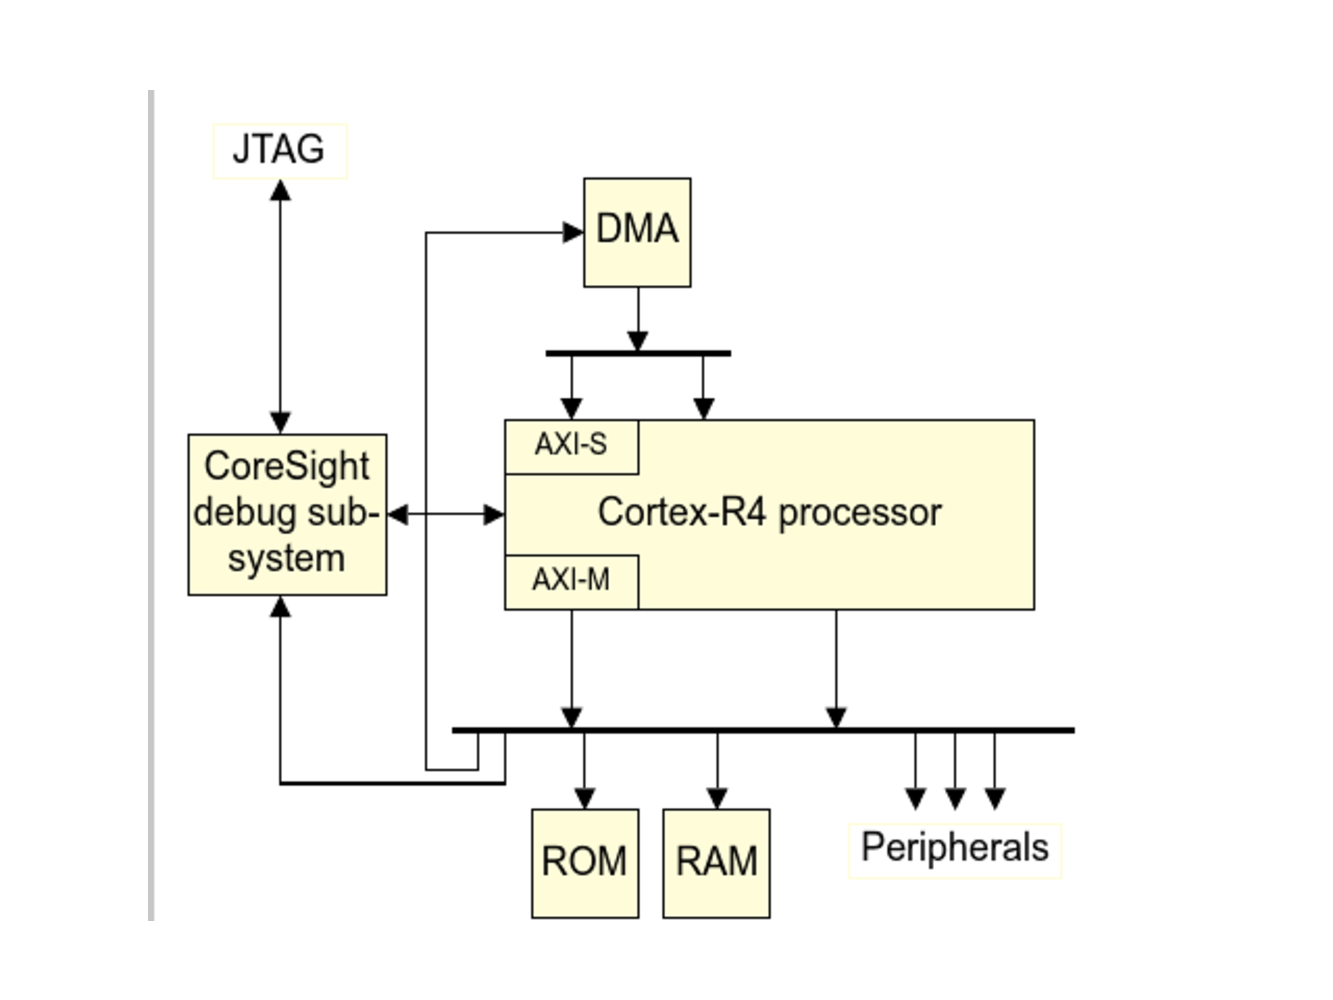
\includegraphics[scale = 0.5]{CortexR4}
\end{figure}

The main features of the Cortex-R4 are listed below:
\begin{itemize}
 \item A Dual issue integer unit with integral coresight logic.
 \item High speed Advanced Microprocessor Bus Architecture(AMBA) and Advance eXtensible Interface(AXI) for master and slave interfaces.
 \item Dynamic branch prediction with history buffer and 4-entry return stack.
 \item Low interrupt latency.
 \item Non Maskable Interrupt.
 \item Optional Floating point unit.
 \item Harvard L1 Memory system with:
 \begin{itemize}{}{}
 	\item Optional Tightly Coupled Memory(TCM) with support for error correction or parity checking.
 	\item Optional caches with error correction codes(ECC).
 	\item Optional ARM-V7R Memory Protection Unit(MPU).
 	\item Optional parity and error correction support for all RAM blocks.
 \end{itemize}
 \item An L2 Memory Interface with single 64-bit master AXI interface and 64 bit slave AXI interface to TCM RAM blocks and cache RAM blocks.
 \item A Performance measuring Unit(PMU).
 \item Vectored Interrupt Controller(VIC).
\end{itemize}

\subsection{Components}

\subsubsection{\textbf{TCM Interfaces}}

TCM Interface for Cortex-R4 are composed of two interfaces, ATCM and BTCM.
An ATCM usually holds the exception handler code that must be accessed at high speed without any cache miss.
BTCM meanwhile holds block of data for intensive operations such as Audio and Video processing.


\subsubsection{\textbf{Power Management}}

Processor includes number of processor features for power management:
\begin{itemize}
	\item Accurate branch and return prediction.
	\item Cache uses sequential access information to reduce the number of accesses.
	\item Extensive use of clocks and gates to disable the inputs to unused functional block.
\end{itemize}

\begin{flushleft}
Cortex-R4 supports 4 different power levels:
\end{flushleft}
\begin{itemize}
	\item \textbf{Run Mode}: The normal mode where all the functionalities of the processor are available.
	\item \textbf{Dormant Mode}:Dormant mode disables with processing logic but not the TCM and cache RAMs. Before entering the mode the processor state is saved to the memory and restored when exiting the mode.
	\item \textbf{Standby Mode}: In standby mode most of the clocks of the device will be disabled, while the device will be kept powered on.
	\item \textbf{Shutdown Mode}: In this mode entire device including cache and TCM logic are disable and should be saved to the external memory.
\end{itemize}

\subsubsection{\textbf{System Reset Levels}}
The processor has following reset inputs: nRESET, PRESETDBGn, nSYSPORESET, nCPUHALT.
Using the combination of given resets following reset modes can be realized: 
\begin{itemize}
	\item \textbf{Power On Reset}:Also known as hard reset or cold reset. Both nRESET and nSYSPORESET are asserted and this is done during initial system reset. This will reset entire system.
	\item \textbf{Processor Reset}:
	Also known as soft reset or warm-reset. nRESET is asserted while nSYSPORESET is set to 1.
	\item \textbf{Halt}: Both nSYSPORESET and nRESET are set to 1 , while nCPUHALT is asserted by setting to 0.
	\item \textbf{Normal Mode}: All three nRESET, nSYSPORESET and nCPUHALT are set to 1. One use case is doing DMA into TCM using the processor.
\end{itemize}

\subsection{Initialization}
Most of the architectural registers in the processor, such as r0-r14, s0-s31 and d0-15 are not reset. Thus these needs to be reset explicitly during the initialization phase.
So of the main activities to be carried out includes: programming registers like stack pointers, processor features and interface initialization and are mentioned below:
\subsubsection{MPU}
If the processor is built with Memory Protection Unit(MPU), before using it program and enable on of its region and enable MPU in system control registers.
If MPU regions are enabled, program them to enable access to TCM regions before using them.
\subsubsection{FPU}
If the processor is build with Floating Point Unit, enable it before accessing VFP instructions. This is done by enabling access to FPU in Coprocessor Access Registers.
Also enable FPU by setting the EN bit in FPEXC(Floating point Exception) register.
\subsubsection{Cache}
If the processor are build with instruction or data cache they must be invalidated before use otherwise the behavior is unpredictable.
If ECC is to be supported for the cache, it must be enabled before invalidating the cache by programming the Auxiliary Control Register. This enabled correct error code or parity bits are calculated.

\subsubsection{TCM}
TCM is not explicitly initialized by Processor and as such should be initialized as per the requirement.
Additionally main instruction may require data to be preloaded into TCM. There are multiple ways TCM memory can be preloaded and are listed below:
\begin{itemize}
	\item The boot code can copy the required data from ROM using the memory routine. For this TCM need to be enabled and separate base address to TCM during copy and normal program execution are provided.
	\item Boot code includes routine to copy data from the Debug Communications Channel(DCC) to TCM.
	\item Processor is put into debug halt state and Instruction Transfer Register(DBITR) is used to transfer data that is executed by the processor and overrides the boot code.
	\item SoC includes DMA device which can directly write the data from ROM code to TCM through AXI slave.
	\item Debug Access Port(DAP) can be used to generate AMBA transactions to write data directly to TCM through AXI slave.
\end{itemize}
Refer to Auxiliary Control Registers to check for initializing TCM with ECC\footnote{Error Correction Code}.
Processor can be pin configured to enable TCM at reset.
\section{CORTEX M0+}
A low area low power 2 stage pipelined architecture for low power modules.\\
compact with total of 56 instructions.\\
Uses AHB lite bus for communication with peripherals and uses 32 bit addressing for a total of upto 4gb of addressable memory.\\
Support two main control modes: Kernel mode and User mode.
User mode can be further divided in to two sub categories of privileged and non-privileged.\\
PSR or Programme status register has 3 main types: Application Program SR, Interrupt Program SR, Exception Program SR.\\
CMSIS Support package provided, which is a a standardized way to access peripheral registers and exception vectors.\\
Memory types can be: Normal, Device, Sharable, Strongly Ordered, Execute Never.\\

Order of execution of the program instructions can be guaranteed by:
\begin{itemize}
	\item Data Memory Barrier(DMB): Assures that the memory operations are completed before next memory operation instruction.
	\item Data Synchronization Barrier(DSB): Ensures that memory operations are completed before start of the next instruction execution.
	\item Instruction Synchronization Barrier(ISB): Ensures that modification to all the instruction before this operation are reflected for all the instruction that executes after this. 
\end{itemize}
Some use case of these memory barriers are:
\begin{itemize}
	\item Vector Table: On update of vector table DMB makes sure further instructions are correctly reflected.
	\item Self Modifying codes: Should make use of DMB followed by ISB.
	\item Memory Map Switching: DSB followed by ISB.
	\item MPU Programming use DSB followed by ISB.
	\item VTOR Programming: While updating vector offset register, use DSB.
\end{itemize}


\subsection{AUTOSAR Specific Features}
This section covers the features of TMS5703137 platform which are significant in supporting AUTOSAR specifications.
\subsubsection{Timing Protection Support}
\begin{itemize}
	\item \textbf{RTI}:\\ Real Time Interrupt(RTI) provides a time tick source to drive the schedule tables in AUTOSAR. 
\end{itemize}
\subsection{Memory Protection Support}
\subsection{Interrupt Vector Table and Peripherals.} % Study of cortex R4 Architecture.

\chapter{Autosar Internals}
\section{Design and Approach}

AUTOSAR provides a standardization of the software stacks that are employed in Automotive systems. It allows collaboration between various partners by standardization of the data exchange format and integration of basic software and application software from various partners on a single ECU via a middleware and across the vehicle network.
AUTOSAR supports broad variety of domains which includes but not limited to:
\begin{itemize}
	\item body/comfort.
	\item driver assistant systems.
	\item powertrain.
	\item chassis control.
	\item occupation and pedestrian safety.
\end{itemize}

\section{OS Internals}

AUTOSAR extends OSEK/VDX Operating systems standards which finds wide adoption in automotive systems.
OSEK OS is an event triggered operating system. This provides high flexibility in the design and maintenance of the system. Event triggering gives freedom of selecting from a wide range of events to drive scheduling at runtime and this includes angular rotation, local timer , global time source, error events etc.
\subsection{BSW Scheduler}
BSW Scheduler provides the basic abstraction for handling of task behavior specific to the timing and control.
AUTOSAR Specification neither provides nor recommends any specific implementation of the BSW Scheduler but specifies the feature set that are to be provided.
BSW Scheduler is not a competing entity to AUTOSAR OS Scheduler, instead it provides following features:
\begin{itemize}
	\item embed BSW modules in AUTOSAR Context.
	\item trigger main processing functions of the BSW Module.
	\item Apply data consistency mechanism for the BSW modules(e.g. Locking mechanisms.)
\end{itemize}
For example, BSW Module provides EnableAllInterrupts and DisableAllInterrupts APIs as a meaning of serializing the execution of the critical sections.
The BSW scheduler files encompasses a SchM.h file providing the abstraction to start the task corresponding to the BSW Scheduler and set of support file which are of the form BSW\_<Module Prefix>.h.
The module specific files are a form of contract to support the data consistency mechanism promised by the BSW Scheduler.
\begin{figure}[h]
	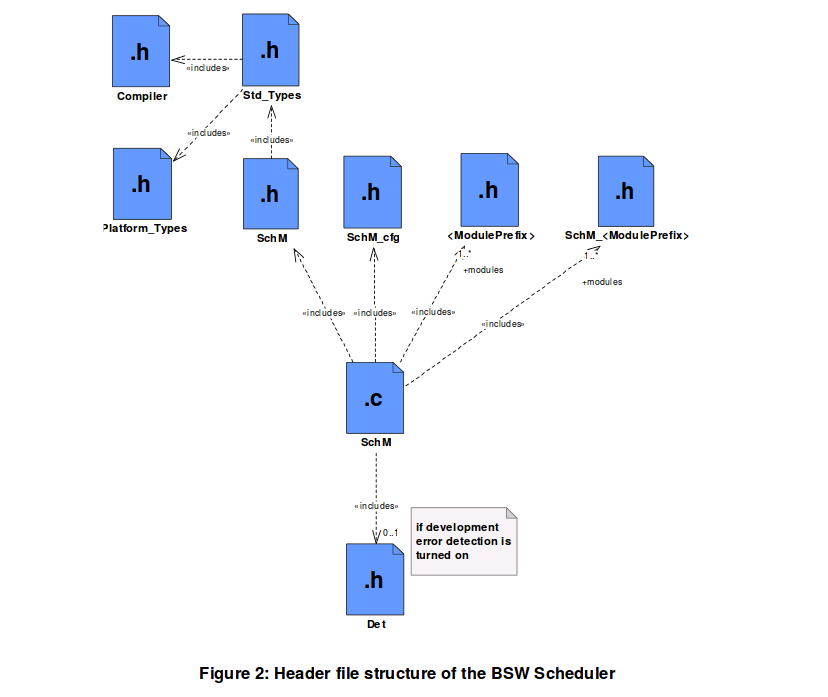
\includegraphics[scale = 0.5]{Pictures/BSW_Schduler.png}
\end{figure}
BSW Scheduler can be implemented as a task that will handle read write operations.
BSW Scheduler cannot invoke the main functions that can enter the wait state.
Thus BSW Scheduler handler the entities, which being the individual actions that can be handled in the context of a task, while the task level control resides with AUTOSAR OS Scheduler.
\subsection{OS Interrupts}
Interrupts under AUTOSAR are classified into cat1 and cat2.
The difference between the two are as follows:
\begin{itemize}
	\item cat1 interrupts are not allowed to make OS calls. The only APIs they can call are to enable and disable interrupts. While cat2 interrupts can call most OS calls, while others are illegal.
	\item cat1 interrupts have lower latency than cat2.
	\item There exists no support for cat1 interrupts from OS, to abstract the interrupt and its handler from the hardware in portable way and is depends on the platform and the tool-chain.
	\item In cat1 interrupt handler there is no need to lock the critical region as it will be shared with task or interrupt of lower priority.
\end{itemize}
Initialization steps for the interrupt handler involves defining vector table and correct entry for handler function.
cat2 interrupt uses ISR macro to define the interrupt handler, advantage of this being, it encapsulates the handler function.
Mutual exclusion in cat2 interrupts are provided by BSW Scheduler in the for of disabling and enabling interrupt sub group.
In case of cat1 interrupts if the mutual exclusion is required, it can be done in terms of disabling all the interrupts. As this seriously affects the overall performance of the system, cat1 region should be kept to minimum.
\subsection{Time Service Module}
Time Service Module is part of the service layer and provides following features:
\begin{itemize}
	\item Time measurement.
	\item Time based state machine.
	\item Timeout supervision
	\item Busy Loop feature.
\end{itemize}
Time Service Module does not sit on top of the timer stack and does not use and provide all the features of GPT Driver.

\subsection{Time Base Manager}
Synchronized time base manager provides APIs to its customers or time bases, which are synchronized with other time bases of the distributed systems, thus acting as a time broker.
Time Base Manager acts as the central module to which provides absolute time of the system. Typical use case include Sensor fusion(Temporal correlation various sensor data.), Event data recording(Temporal correlation of the logs while reporting on system crash or on detection of an anomaly), and diagnostic event storage.
The customers to the Time Base Manager can be triggered or active. AUTOSAR OS is currently supported as a triggered customer.
A Global time network consists of atleast one Time master and atleast one Time Slave. \\
Figure below shows a representation of such a global time network.

\noindent%
\begin{minipage}{\linewidth}% to keep image and caption on one page
	\makebox[\linewidth]{%        to center the image
		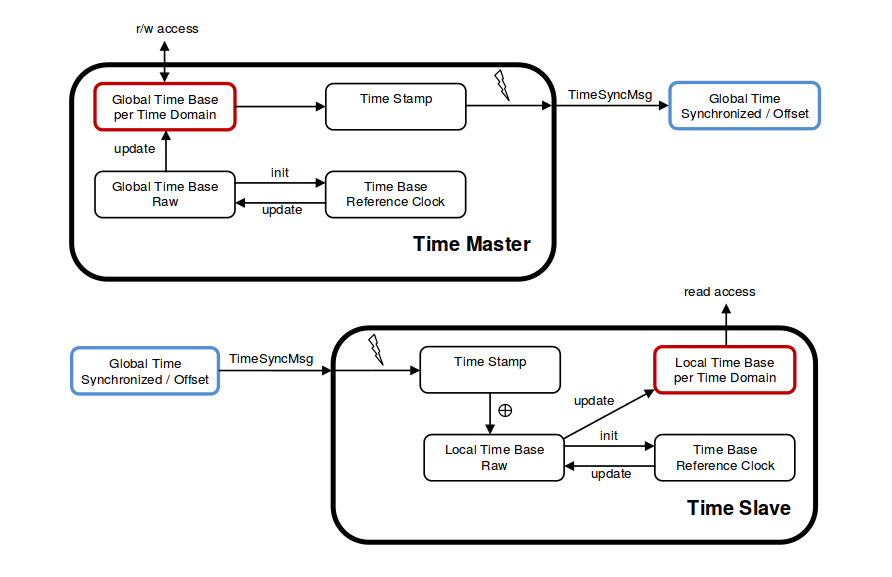
\includegraphics[keepaspectratio=true,scale=0.5]{Pictures/Global_Time_Base.png}}
\end{minipage}

Two different sets of time bases are provided. Time Domains 0-15 are synchronized time bases while Time Domains 16-31 are offset time bases.

\subsection{Core OS Specifications}
In AUTOSAR systems internal communication is provided by RTE or COM at least one of which will be present in the ECUs.
AUTOSAR OS thus when used in an AUTOSAR system does not need to support communication.
One of the key component AUTOSAR OS extends on OSEK/VDX is Schedule tables.
In OSEK it is possible to provide statically defined activation mechanism using an OSEK counter and alarms. To provide runtime modification of the activation, it is necessary to maintain synchronization between the alarms.
Schedule table provides a solution to this issue of synchronization by providing an encapsulation to the statically defined expiry point.
In a schedule table an expiry point corresponds to one or more actions that should occur in the system and corresponds to a fixed offset from the beginning of a schedule table.
Each schedule table is defined by a set of ticks and the os module will iterate over the ticks and invoke appropriate actions at expiry points. \\Figure below shows an example of schedule table.\\
\noindent%
\begin{minipage}{\linewidth}% to keep image and caption on one page
	\makebox[\linewidth]{%        to center the image
		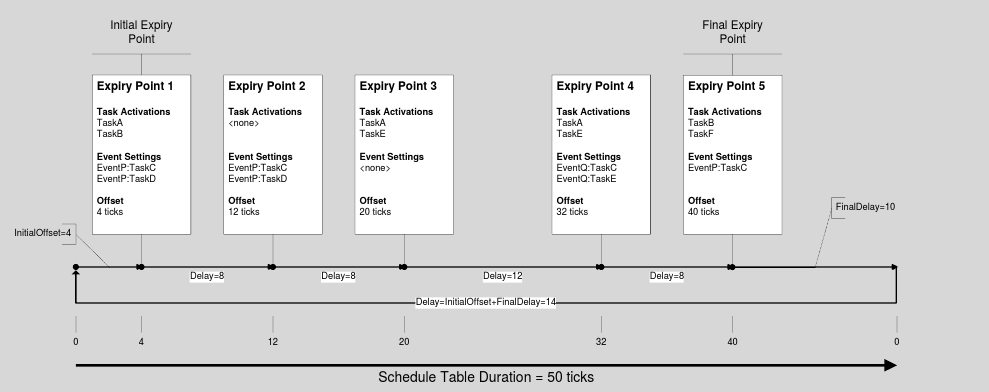
\includegraphics[keepaspectratio=true,scale=0.5]{Pictures/Schedule_Table.png}}
\end{minipage}


 
 % Study of cortex R4 Architecture.

\chapter{Literature Survey}
\section{Adaptive Variable Tasks}
\subsection{Elastic task model for Adaptive Rate Control}
A novel periodic task model is proposed in which tasks periods are provided with elastic coefficients. Under this approach tasks can change there execution rate to provide different Quality of Service(QoS).
To simplify the schedulability analysis simple assumptions are taken, as is the case with RM and EDF. For which tasks with cyclic execution and fixed demand are considered.
But this assumption are too restrictive for application for which timing constraints can be more flexible and dynamic.
Works have been done to done theoretical support to such tasks using probabilistic guarantee, capacity reservation based approach or by providing an upper bound on the job chains with variable executions.
Varying tasks rate provides the possibility of handling a graceful task degradation rather than outright rejection of some tasks.
A number of approaches have been proposed for dynamic and static load balancing to handle overload conditions. In \textit{"QoS Negotiation  in  Real-Time Systems  and  Its  Applications to Automated Flight Control"} QoS is proposed as a set of negotiation options based on reward and rejection penalties.\\
This Paper tries to propose a generic way for tasks to change there execution rates and provide varying QoS under different condition.
The elastic task model works by compressing the taskset under overload condition. The compression of tasks is handled depending upon the elastic coefficient \textit{e}. Another advantage of elastic task model is when considering a new task into otherwise schedulable task set. Under a rigid task model this will not be feasible, but by using elastic task compression the new task could be accommodated.\\
The basic algorithm used to tune the elastic tasks is given below:


\begin{minipage}{\linewidth}% to keep image and caption on one page
	\makebox[\linewidth]{%        to center the image
		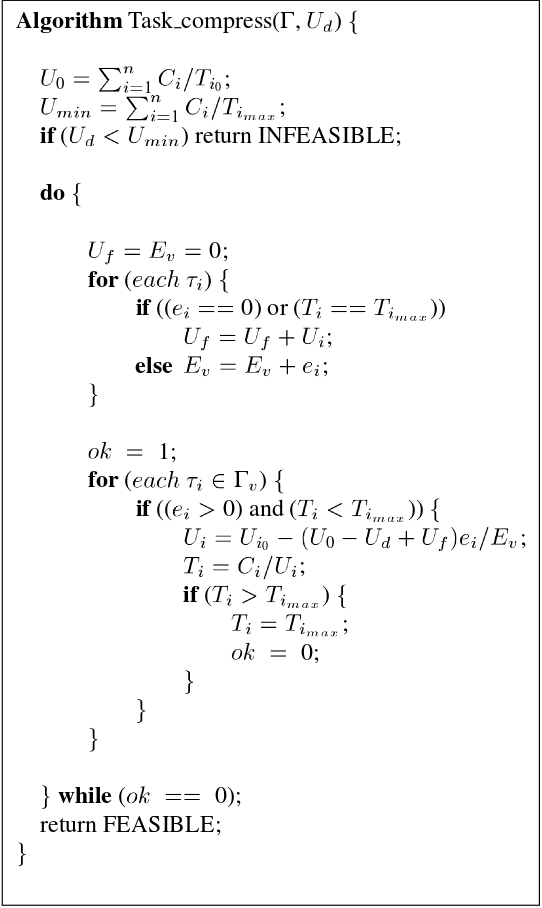
\includegraphics[scale=0.5]{Pictures/Elasic_algo.png}}
\end{minipage}

\subsection{Towards runtime adaptation in AUTOSAR}
This paper put forwards a method to extend the AUTOSAR mode management to implement runtime adaptation.
To realize runtime adaptation in AUTOSAR relocation of software components at runtime is required, which in turn is based on computation of adaptations during runtime.
To meet the Adaptation requirements the new model tries to meet to following challenges.
\begin{itemize}
	\item Real time requirements.
	\item Self describing components.
	\item Scheduling.
	\item ECU Independent addressing.
\end{itemize}
The runtime adaptation is implemented by two components: Adaptation Service and Adaptation Manager.
Relocating software requires control over starting and stopping of AUTOSAR Software Components, this is done by extending the system by a runtime control based on MAPE(Monitor, ANalyze, Plan and Execute) cycle.


\begin{minipage}{\linewidth}% to keep image and caption on one page
	\makebox[\linewidth]{%        to center the image
		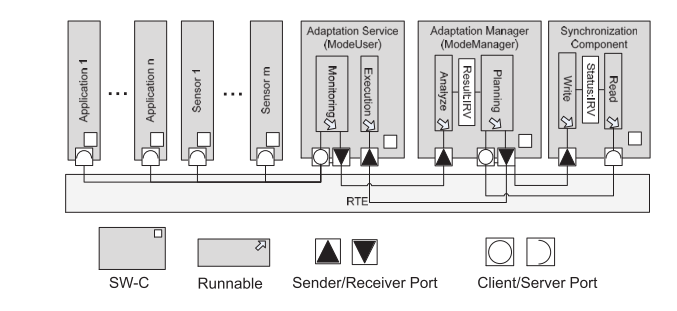
\includegraphics[scale=0.5]{Pictures/Adaptation_Manager.png}}
\end{minipage}
\begin{itemize}
	\item \textbf{Monitoring Mechanism} : Monitoring unit extends the mode manager. A request to change the mode to meet the new requirements is initiated to Mode Manager.
	\item \textbf{Analyze}: Mode manager does the analyze and planning phase. A single adaptation manager can exist in entire automotive network or to properly extend Mode manager, one Adaptation Manager shal exist per ECU. This also has the added benefit of redundancy avoiding single point of failure.
	\item \textbf{Synchronization Mechanism}: Mode Manager shall notify the Synchronization manager of the changed execution and will synchronize it across the ECUs in network.
	\item \textbf{Real-Time requirements}: The Adaptation mechanism implemented shall always be determined with respect to the component timing requirement.
	\item \textbf{Self-Describing components}: In order to check for the timing requirements the components shall publish the attributes needed for runtime verification such as end to end deadline.
	\item Scheduling: EDF Scheduling to provide better efficiency.
\end{itemize}
\subsection{Fast and Tight Analysis of AUTOSAR Schedule Tables.}
Proposes how to quantify the response time of the schedule table driven task set considering the offset and resource based priority threshold interference.
Two different analysis of rta and maximum time to release of a given task under a given time frame \textit{t}, as well as maximum time to completion of the given task is put forward.
First method being tight fit while the second method is an approximate estimation of the above mentioned parameters.
\subsection{Evaluation and Implementation of Mixed-Criticality Scheduling Approaches for Periodic Tasks}
The paper proposes a quantitative comparison of MC Approaches including: Priority assignment, Period transformation and Zero-slack scheduling.
Zero slack scheduling is improved by addressing two previously known issues: How to accommodate execution of a task after its deadline and how to handle previously unknown interferences.

\subsection{Towards the design of certifiable mixed-criticality systems.}



% Paper on fault injection mechanisms: Authors Thorsten Piper et.al

\section{On the effective use of Fault injection for the assessment of AUTOSAR} % Major section
%------------------------------------------------
\subsection*{Key Idea} % Sub-section
AUTOSAR safety standard ISO26262 strongly recommends usage of the fault injection standards, but no definite mechanism exists for enforcing the same.
Representation of the faults using the standard fault models e.g. bit flips and data type based corruption are not sufficient to model real time behavior.
The existing Fault Injection framework GRINDER is extended to support AUTOSAR and an assessment is provided.
%-----------------------------------------------
\subsection*{Width and scope} % Sub-section
Provide open source and ready to use framework to do Fault Injection. Dependability  assessment on existing AUTOSAR timing monitor safety mechanism for identifying 
deficiencies and guidelines for derivation of special fault models, injection mechanisms and locations based on abstract AUTOSAR and ISO26262 fault models.
Eariler approach mentioned include: Lanigan et.al. and Baugarten et al. First approach being based on VECTOR CaNoe and second approach used anotated SWC Component to 
introduce fault ports. Another approach is pre implementation testing using UML or AADL, in this failure level are assumed and the effect on model analysed.
Vedder et. al extended property based testing to AUTOSAR. Here automated test cases were generated from a pre specified property files.

Hardware based FI: Modeling hardware error such as CAN bus failure, or NVRAM failure through corrupted CRC. Hardware based FI fails to handle component interaction and
dependability property.
Software based FI: e.g. BeSafe framework to intercept SWC calls and fuzzing error models to check resilience of SWC. GOOFI-2 to evaluate bit flip cases and  MODIFI to check model
at Simulink level.\\
\textbf{Note:} Simultaneous fault models with multiple points of failure completely missing from AUTOSAR standards.

%------------------------------------------------

\subsection*{Experimental approach} % Sub-sub-section
\begin{itemize}
	\item \textbf{Configuration}: Target is instrumented with injectors and detectors.
	\item \textbf{Execution:} The target system is executed till the injection of fault and the perturbation data is successfully completed.
	\item \textbf{Evaluation:} The logs and traces are collected.
	GRINDER extended to AUTOSAR by providing a target specific implementation of TargetAbstraction Class with which GRINDER interacts during FI.
\end{itemize}
A general overview of the architecture is given below.
\begin{figure}
\begin{center}
	\centering
	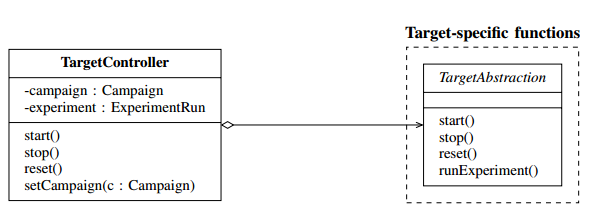
\includegraphics[width=400pt]{Pictures/Grinder_Extension}
	\caption{Abstract Target representation of GRINDER}
\end{center}
\end{figure}

\begin{figure}[H]
	\centering
	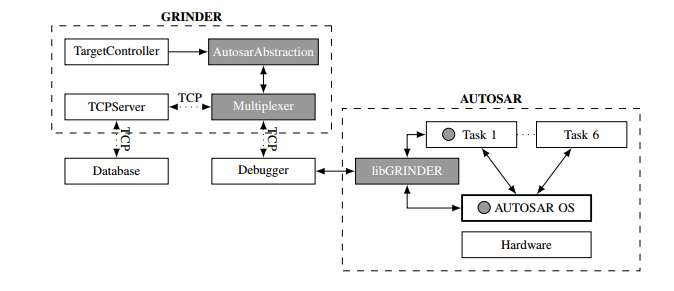
\includegraphics[width=400pt]{Pictures/GRINDER_Arch}
	\caption{GRINDER new arch.}\label{visina8}
\end{figure}
%------------------------------------------------

A case study is further done on Adaptive Cruise Control module. 
\begin{figure}[H]
	\centering
	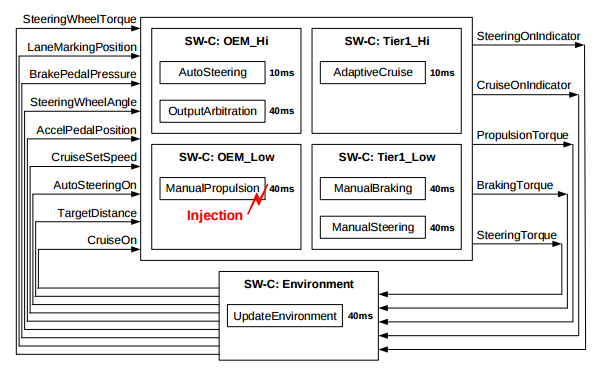
\includegraphics[width=400pt]{Pictures/ABS}
	\caption{ABS Module architecture}\label{abs}
\end{figure}


Four different scenarios tested:
\begin{itemize}
	\item Task timing error: Assess the correctness of the error detection and error mitigation of execution time monitoring. Analyze the propagation of the error with and without the presence of the timing errors.
	\item Interaction between the execution time monitoring and resource lock timing monitoring. Assess correctness and robustness of the mechanisms.
\end{itemize}

The task selection for monitoring ABS is shown below:
\begin{figure}[H]
	\centering
	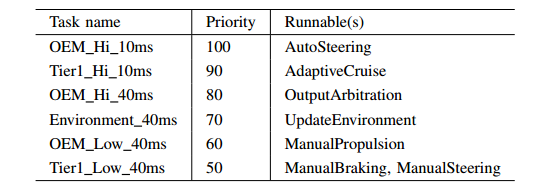
\includegraphics[width=400pt]{Pictures/Task}
	\caption{ACC task setup}\label{abs}
\end{figure}
\subsection*{Conclusion} % Sub-sub-section
Detailed description of scenarios, A good framework to test the mechanism of fault injection and different failure scenarios.
Can be used with possible change to JTAG interface to FTDI interface. Can be implemented as part of the eclipse plugin as as schedulability and testing mechanism.

\subsection*{Links}
http://www1.deeds.informatik.tu-darmstadt.de/External/PublicationData/1/edcc-2015.pdf


%--Adaptive runtime shaping for mixed criticality systems: Biao Hu et.al.
\section{Adaptive Runtime Shaping for Mixed-Criticality Systems}
\subsection*{Key Idea}
Presents an approach to adaptively shape the inflow workload of low-critical tasks based on actual demand of high critical tasks on runtime. Compared to the shaping of the offline bound low-critical tasks event delay is reduced and system utilization is improved.
\subsection{Width and Scope}
Main contributions are:
\begin{itemize}
	 \setlength{\itemsep}{0pt}
	 \setlength{\parskip}{0pt}
	 \setlength{\parsep}{0pt} 
	\item An adaptive scheme for shaping the low critical workload.
	\item A light weight mechanism with complexity of \textit{O(m.log(n))} to refine the shaping bound.
	\item Experimental results to show the efficiency.
\end{itemize}
This work build on three main approaches:
\begin{itemize}
	\item Real-Time interface analysis: Connecting real time interface design and calculus.
	\item Workload prediction: Real time calculus models task activation as event, arrival curves originating from network calculus provide an upper and lower bound on number of arrival events. Prediction method based on historical arrival data. Arrival curve predicted by several stair case functions for tighter prediction.
	\item Runtime shaping: Shapers often used in regulating packets in network. Greedy mechanism for shaping in real time systems. FPGA based shaping mechanism.
\end{itemize}

\subsection*{Experimental Approach}
Task generation using UUnifast mechanism.
Experiments done on MATLAB Based on RTC Tool box(Theele et.al), mainly three different shaping mechanisms are compared.
\begin{itemize}
	\setlength{\itemsep}{0pt}
	\setlength{\parskip}{0pt}
	\setlength{\parsep}{0pt} 
	\item Shaping by offline computed bound.
	\item Shaping by backward derivation online.
	\item Shaping by proposed lightweight scheme.
\end{itemize}
\subsection*{Conclusion}
TMD
\subsection*{Links}
http://www6.in.tum.de/Main/Publications/Biao2015EMSOFT.pdf

%Deadline Analysis of AUTOSAR OS Periodic Tasks in the Presence of Interrupts: Yanhong Huang et.al
\section{Deadline Analysis of AUTOSAR OS Periodic Tasks in the Presence of Interrupts}

\subsection*{Key Idea}
Provide an abstract framework to determine if the given periodic task will miss its deadline in the presence of interrupts.
Rather than bounding interrupts for given time. Proposes a mechanism to bind the timing calculation to maximum number of interruption allowed to a given task from interrupts.(e.g. The task will meet deadline as long as the number of interrupts is at most n.)
\subsection*{Width and Scope}
Provides a mean to abstract representation of the maximum number of interruption allowed to a task.
Assumptions part of the approach:
\begin{itemize}
	\setlength{\itemsep}{0pt}
	\setlength{\parskip}{0pt}
	\setlength{\parsep}{0pt} 
	\item Tasks are periodic and are implicit in nature with deadline equal to period.
	\item Any task activated by ISR2 will execute and terminate before the end of the ISR.
	\item Resource locking and blocking to the tasks due to it are not considered.
\end{itemize}
Mentions two independent healthiness concept: Task that is not interrupted and tasks that are interrupted.
\begin{figure}[H]
	\centering
	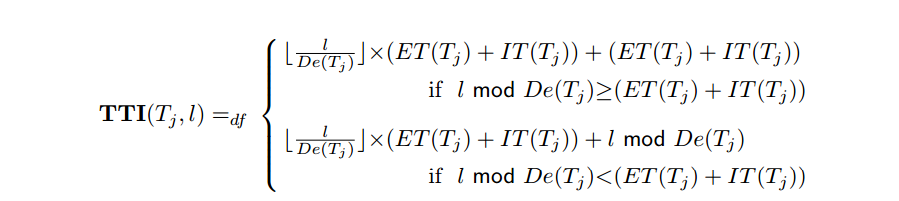
\includegraphics[width=400pt]{Pictures/Autosar_TTI_Bound}
	\caption{Timing Bound formula}\label{abs}
\end{figure}
\subsection*{Experimental Approach}
Experiments done on Mathematica. Total slack available then split to interrupt times.
\subsection*{Conclusion}
Calculate the slack, split it in terms of ISR time.That's main idea.
\subsection*{Link}
http://haslab.uminho.pt/jff/files/2013-deadlineanalysisautosar\_os.pdf
%Mitigating Timing Error Propagation in Mixed-Criticality Automotive Systems: Thorsten Piper et al.
\section{Mitigating Timing Error Propagation in	Mixed-Criticality Automotive Systems}
\subsection*{Key Idea}
ISO26262 stipulates freedom from interferences, i.e, error should not propagate from low to high criticality tasks.
Different from indirect protection of the critical tasks, approach provides direct low overhead protection to high critical tasks by introducing the concept of preemption budget.
\subsection*{Width and Scope}
Introduces the concept of Preemption Budget(PB) and its specifies the maximum amount of time for which a critical task can be preempted. This is very much similar to the concept of Adaptive Mixed Criticality scheduling with deferred Preemption(AMC-DP), which specifies a minimum amount of time for which the task has to be run without any preemption.
Timer based approach, For critical task that are active in the run queue timer is started to limit the earliest expiring preemption time. Once the preemption time is depleted the task is moved up the run queue and made to execute for rest of its budget.
Handles Transient error runthrough (A mechanism similar to tolerence, where tasks are allowed to stretch the budget). Transient error run through is allowed under PB due to the slack available.
\subsection*{Experiments}
Study of Transient and Permanent fault cases for ACC tasks.
PBM Budget monitoring implemented under AUTOSAR, measurement made for static code size increase due to the implementation and the overhead incurred due to the budget monitoring.
\subsection*{Conclusion}
An alternate take on AMC-DP and Tolerance limit based approach implemented and evaluated to show low overhead.
%A Heuristic algorithm for mapping autosar runnables to tasks.
%\textbf{https://hal.archives-ouvertes.fr/hal-01341785/document}
\section{A Novel heuristic Algorithm For Mapping AUTOSAR Runnables To Tasks.}

\subsection*{Key Idea}
Runnables represents the internal behavior of SwC in AUTOSAR and are the smallest pieces of the code to be scheduled.
All runnables are triggered in response to an event such as timing event, data receiving or operations invoking the runnables.
Key question is deciding upon how many tasks are required to represent a set of runnables, how to define priority and how to define activation offset and execution order of the tasks.\\
Prominent methods of grouping the runnables to tasks are:
\begin{itemize}
	\item \textbf{{Periodic Solution}}: Runnables with same period are assigned to one task. WCET of the task is sum of the WCET of all the runnables mapped to it.
	\item \textbf{Multiple Periodic Solution}: In this approach period of the task is the shortest period among different runnables mapped to it.
	\item \textbf{Arbitrary Periodic Solution}: In this approach runnables with different approach are mapped to same task using their activation offset. period of the task is GCD of all the runnables mapped to it.
\end{itemize}
For APS and MPS system schedulability may be guaranteed using Rate Monotonic Period Assignment(RMPA) or Deadline Monotonic Period Assignment(DMPA).
Currently multiple approach to mapping exists, including use of MILP, Simulated Annealing and Genetic algorithm based approach.

\subsection*{Width and Scope}
Using Audsley's approach to sort out the tasks among different schedule frames with constraint of width of the frame and the deadline of each of the runtimes.

\subsection*{Conclusion}
Neat way, but practicality is limited, as usual runtimes of tasks are grouped to common schedule tables as there functionalities are important.
\section{Scheduling Algorithms and OS Support for RTS.}
\subsection{Key Idea}
An overview of the scheduling support in real time systems and subsequent use cases in commercial of the shelf RTOS.
Three main type of scheduling paradigms are discussed:
\begin{itemize}
	\item Static table driven approaches.
	\item Static priority driven approaches.
	\item Dynamic planning based approaches.
	\item Dynamic best effort approaches.
\end{itemize}
Discussed are table driven scheduling, priority based preemptive scheduling, cyclic scheduling.
Cyclic scheduling resembles the schedule table approach used in autosar based systems. Here tasks are assigned one of a set of harmonic periods. 
If purely priority driven approach is used, by using task deadlines as priorities, and without any planning, task would be preempted at any time.
So unless the deadline is reached or task completes, whichever comes first, It is not possible to know if the task constraints are met.
So worst case performance analysis of such a task system is necessary.\\
When tasks are acted upon by parameters other than priority like resource requirements heuristics based approach on branch and bound are necessary.
\subsection{Ideas}
Priority categorization of I/O bound and CPU bound tasks in the context on non-realtime systems.
\begin{itemize}
	\item In addition to being intuitive, static priority assignment forgoes re-computation of the priority at runtime.
	\item Similar to EDF, another dynamic approach to scheduling is based on laxity, or least laxity first scheduling.
	\item Although feasibility checking on schedulability is made easier by preemption, most schedulability analysis ignores the dispatch cose associated with scheduling, which can be significant depending upon the task characteristics.
	\item Dynamic planning based algorithm: OCBP can be considered a variant of this approach. In this approach a task is guaranteed by constructing a plan for the all the tasks that are available at its possession at the given time.
	\item Different mechanisms to dynamic planning algorithms exist: Focused addressing, bidding algorithm, flexible algorithm or a combination of bidding/focused algorithm.
	\item Dynamic best effort algorithm: Used in most of the multicore real time systems. Example being earliest deadline first and the least laxity first algorithms.
\end{itemize}
\subsection{Comclusion}
Paper is representation of work in the area of scheduling and operating system support for the same.


%Towards runtime adaptation in AUTOSAR.
\section{Automotive Control System Notes}

\subsection{Review of Engine Modelling.}
\subsection{Review of Vehicle Dynamics.}

\section{On Scheduling Tasks with Quick Recovery from Failure}
% CM Krishna and Kang G Shin
Proposes a dynamic programming algorithm that ensure that backup or contingency schedules can be embedded in original primary schedule so that hard real time deadlines continues to be met in the face of upto maximum number of processor failure.
\subsection*{Key Idea}
The main aim of this approach is to create a limp mode schedule mechanism, where in spite of failure to few available processor nodes, system is able to meet its real time constraints.
The optimization criterion uses cost function, which corresponds to the feedback delay incurred in the control network. \\
Tasks are run periodically and each instance is known as version. 
Multiple copies of versions are called \textit{clones}. There are two types of clones: primary and ghost. A ghost clone is a backup copy which remains dormant until it is activated to take the place of corresponding primary or another ghost whose processor has failed.
\subsection*{Concepts}
An algorithm \textit{P} is considered consisting of two components: \textit{P1} and \textit{P2}.
P1 finds the optimal allocation of tasks to processor and also optimal schedule by calling P2 which is an optimum scheduler for uniprocessor systems.
\subsection*{Problem Statement}
Develop and algorithm Q, that can be used in conjunction with P1 and P2 to obtain an optimal schedule when enough ghosts are incorporated into the schedule to handle N$_{sus}$ processor failures.\\
Schedules designed are considered to be locally preemptive and globally non-preemptive to reduce interconnect overloads.\\
\begin{minipage}{\linewidth}% to keep image and caption on one page
	\makebox[\linewidth]{%        to center the image
		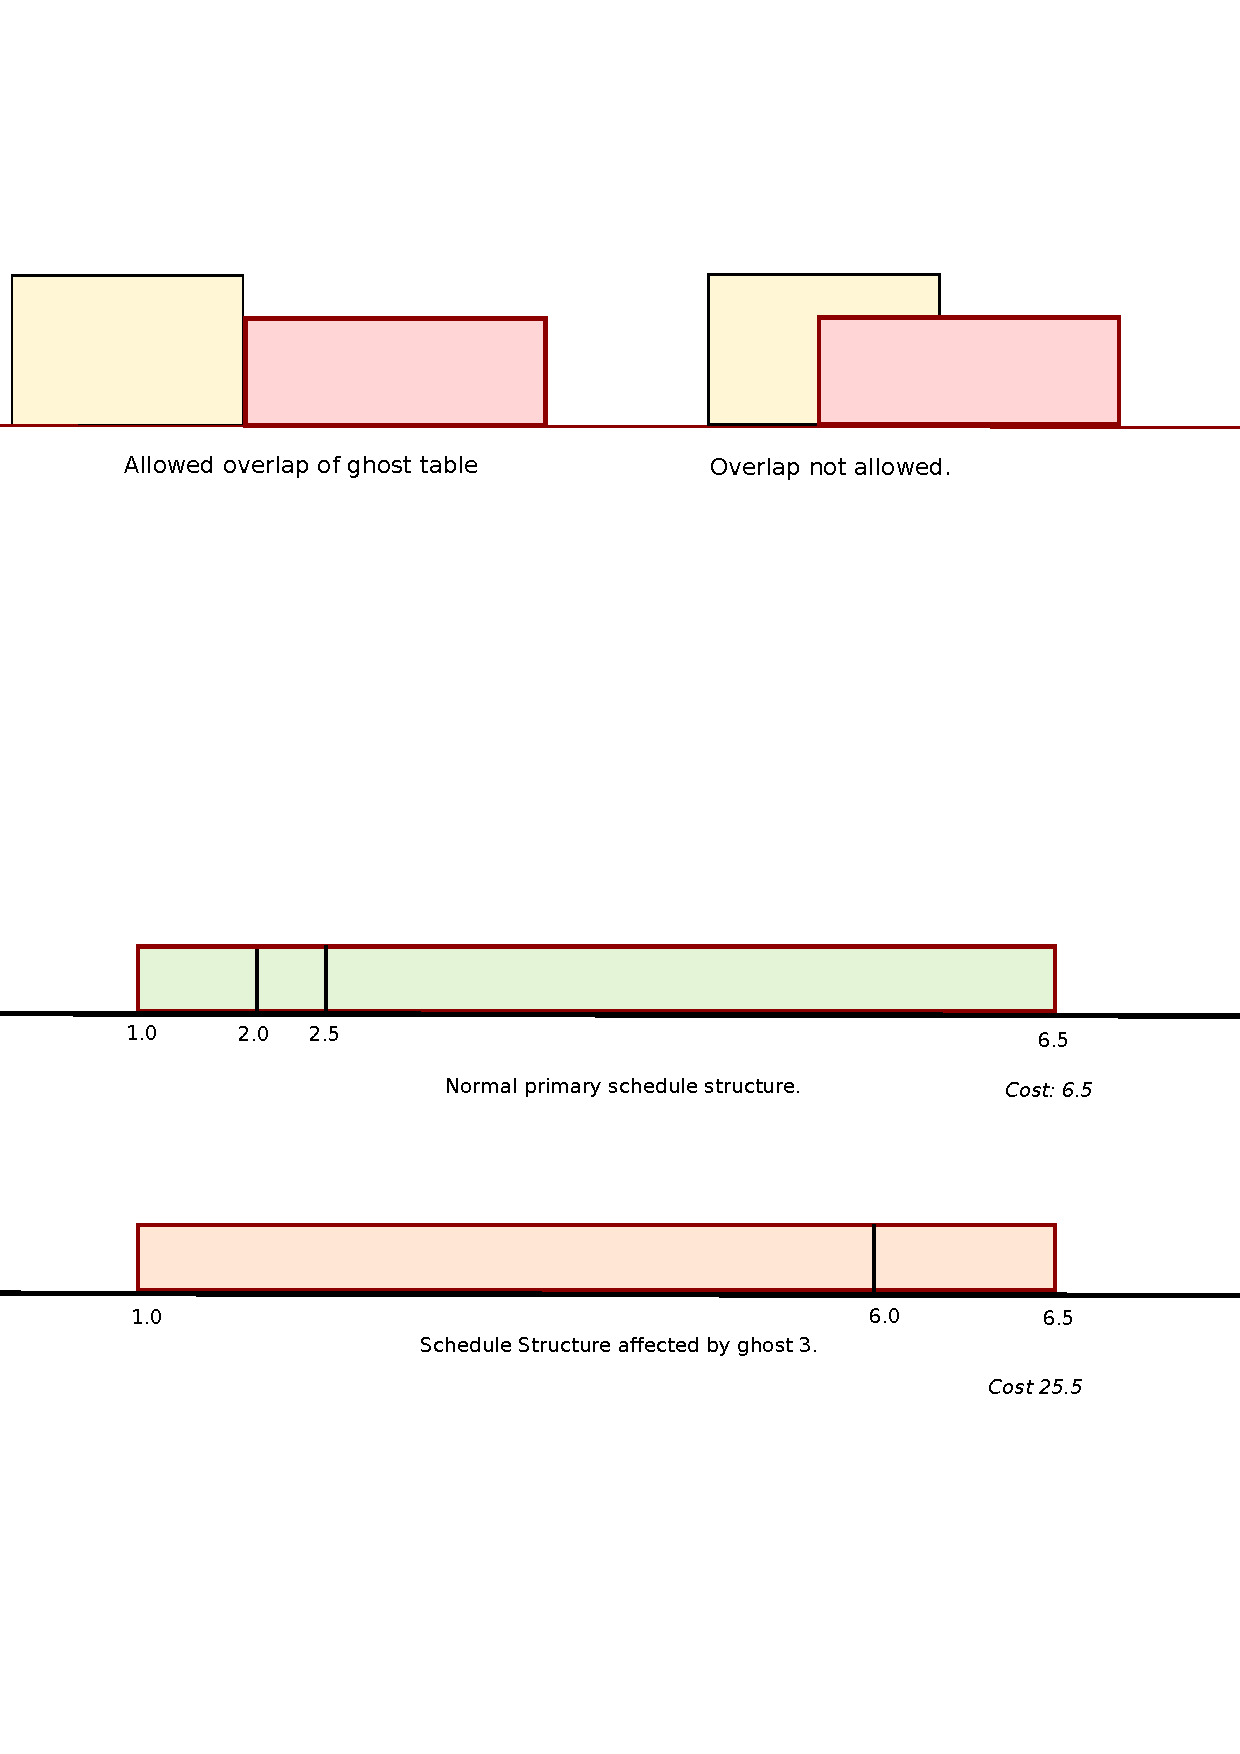
\includegraphics[scale=0.52]{Pictures/paper08_schedule.pdf}}
\end{minipage}
\\
\subsection*{Scheduling mechanism}
Dynamic programming to find the slack holes existing with in the primary schedules. Now do compactness to generate extended holes to schedule ghosts, such that compactness allows the primary tasks to meet there deadlines. In a way similar to the elastic scheduling approach where each task is compacted with restriction being the elasticity coefficient.
\subsection*{conclusion}
A partitioned schedule table driven approach with slack stealing across the cores in case of failure. Its main difference from traditional slack stealing is that, the alternate schedule tables are kept on other processors to be activated in case of failure of the primary schedule. And the activation of the ghost table should not in any way act upon the primary table on the given core.
\section{On the Scheduling of Mixed-Criticality Real-Time Task Sets}

\subsection*{Main Idea}
This paper introduces the concept of Zero slack scheduling, In zero slack scheduling the task consist of two execution modes: normal and critical. When a task is unable to meet its budget demands in normal mode, it switches to critical mode at the last instance at which it is able to meet the demand in critical mode.


\chapter{Automotive control systems}
\section{Power-Steering Control Architecture for Automatic Driving}
A two layered control architecture to automatically moving the steering wheel is presented.\\
\subsection*{Overview}
\begin{itemize}
	\item Two layer control architecture, first layer is designed to calculate the position of the steering wheel at any time based on fuzzy logic.
	\item The second layer is a classic control layer that moves the steering wheel to the position predicted by the first layer, monitored by Real-Time Kinematic Differential Global Positioning System(RTK-DGPS).
	\item Comparison is done for the performance of the implementation to human driver. 
\end{itemize}

\subsection*{Key points}
\begin{itemize}
	\item There are two ways to implement automatic steering control, Imitating a driver or using dynamic models of car and control methods based on linear control theory.
	\item  the main contribution
	of this work is the combined use of a PID and a fuzzy controller
	in a cascade-control scheme, and its application to regulate the
	steering wheel of a mass-produced vehicle.
	\item The sensor input comes from GPS receiver at a frequency of 10Hz.
	\item Each measured value is compared with reference GPS trajectory. Two input variables are gathered from this comparison: the lateral and angular errors.
	\item A Fuzzy control ingests these two inputs to generate target steering turning command.
	\item Fuzzy control performs three main functionalities: fuzzification, inference, defuzzification. 
	\item Two different driving conditions are handled. Straight road and curved road.
	\item Straight road steering angles are considered short and fast reactive while curve is considered higher steering angles and slower reaction.
	\item Steering angle is limited to 2.5\% on straight road. While in curve mode the angle is not limited.
	\item Center-of-area method is used for defuzzification.
	\item Each crisp value, which is left or right steering output is multiplied by square of weight and averaged over sum of weights.
	\item The weights are calculated using Mamdani's rule inference method.
	\item The trajectory control defined above is fed to a PID controller that is tuned on the basis of Zeigler-Nichols method and further tuned experimentally, proportional, integral and derivative gains were adjusted to yield an overdamped closed-loop response.
	\item Proportional, integral and derivative gains were set to 20, 50 and 1000 respectively.	
\end{itemize}

\subsection*{Pseudo codes}
\begin{algorithm}
	\caption{First layer Fuzzy Controller}\label{fuzzy}
	\begin{algorithmic}[1]
		\Procedure{Fuzzy\_Rule()}{}
		\If{\textit{Angular\_Error == Left} || \textit{Lateral\_Error == Left}} \Return Right
		\EndIf
		\If{\textit{Angular\_Error == Right} ||\textit{Lateral\_Error == Right}} \Return Left
		\EndIf
		\EndProcedure
	\end{algorithmic}
\end{algorithm}

\subsection*{reference}
Paper Link:
\section{Predictive Active Steering Control for Autonomous Vehicle Systems}
A Model Predictive Control (MPC)
approach for controlling an Active Front Steering system in an
autonomous vehicle is presented.
\subsection{overview}
\begin{itemize}
	\item Early work on active safety focused on improving longitudinal dynamics part of the motion, in particular, on more effective braking system(ABS) or traction control system(TCS). ABS increases the braking efficiency by avoiding the lock of braking wheels. TCS prevents wheel from slipping at the same time improves vehicle steerability and stability by maximising the tractive and lateral forces.
	\item This was followed by work on vehicle stability control system known under different acronyms such as Electronic Stability Program(ESP), Vehicle Stability Control(VSC), Interactive Vehicle Dynamics(IVD), Dynamic Stability Control(DSC) etc.
	\item Other subsystem that are being investigated involves 4 wheel steering, active steering, active suspension, active differential etc.
	\item Focus on control of the yaw and lateral vehicle dynamics via active front steering.
	\item The control input is the front steering angle and the goal is to follow the desired trajectory or target as close as possible while fulfilling
	various constraints reflecting vehicle physical limits and design
	requirements.
	\item The future desired trajectory is known only over
	finite horizon at each time step. This is done in the spirit of
	Model Predictive Control.
	\item Two different formulation of Active Front Steering Model Predictive Control is presented and analyzed.
	\item Non Linear Vehicle model to predict future evolution of system. A non linear optimization problem is solved at each computation instance.
	\item Second approach uses a sub-optimal MPC Controller based on successive on line linearization of the non-linear model. Approach also known as LTV(Linear Time Varying Model.)
\end{itemize}
subsection{Key Ideas}
\begin{itemize}
	\item Bicycle model for the vehicle.
	\item Control system consisting of trajectory planning - low level control system and actuator system.
	\item Guidance and Navigation Control System - Trajectory-Mode Generator + Trajectory-Mode Replanning + Low Level Control System.
	\item Trajectory-Replanner :- Receding Horizon Control design.
	\item Vehicle-Model :- Rear centered kinematic model with acceleration, steering, speed, steering rate and rollover constraints.
	\item Computation heavy non-linear optimization model.
\end{itemize}
\subsection{Conclusion}
Too complex a model to be used for analysis of the scheduling patterns.

\chapter{Proposed Design}
\section{Scheduler Design}

\chapter{Test and Measurement Methodology}
\section{FTQ/FWQ}
%https://asc.llnl.gov/sequoia/benchmarks/FTQ_summary_v1.1.pdf
%ASC Sequoia Benchmark Codes: https://asc.llnl.gov/sequoia/benchmarks/

The FTQ/FWQ benchmarks measure hardware and software interference or 'noise' on a node from the applications perspective.\\
FWQ(Fixed Work Quanta) and FTQ(Fixed Time Quanta) runs on each core and hardware thread within a single node via pthreads. FWQ continuously  measure the time taken to execute a fixed amount of code. FTQ repetitively works for a fixed amount of time and measure the amount of work done in the given time period.\\
Due to the fixed work approach of FWQ, the data samples can be used to compute useful statistics (mean, standard deviation and kurtosis) of the scaled noise (sample time minus the minimum work time and scaled by the minimum work time). \\
Due to the fixed time quanta approach of FTQ, the work data can be processes with a Fast Fourier Transform (FFT) in order to determine the temporal frequency of software interference.  This is an extremely useful tool to find sources of periodic interference such as scheduling intervals, the regular operation of daemons, etc. 

\section{Time measurements on TI TMS-570-LS3137}
The main approaches to logging under ti hercules platform are discussed here.

\section{A Practical Approach to the Simulation of Safety-critical Automotive Control Systems considering Complex Data Flows}

\subsection*{overview}
\begin{itemize}
	\item Issue of determining end to end latencies in systems composed of functional and dysfunctional modes of operations.
	\item Depending on required safety level the complexity of implementation varies.
	\item Development consists of finding the real time bottlenecks, verifying and deploying, and as such is complex.
	\item Aims to provide virtual integration of system early in development stages.
\end{itemize}
\subsection*{Main points}
\begin{itemize}
	\item Important task is planning execution of tasks and ISRs.
	\item Model based simulation of various execution scenarios to determine the worst case overhead of task executions.
	\item Event chain used to specify a sequence of execution and data flow, subject to RT requirement.
	\begin{minipage}{\linewidth}
		\centering
		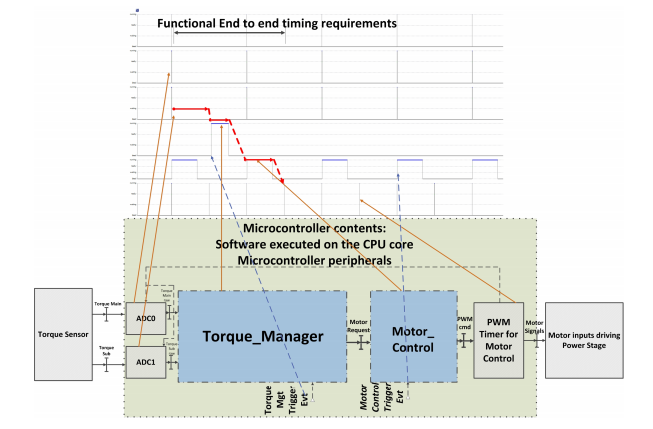
\includegraphics[width=13cm]{Pictures/Event-chain.png}
	\end{minipage}
	\item Initially data flow between hardware and software components at system level were modeled using flow port concept of \textit{SysML}.
	\item Formalized model analyzed using INCRON tool-suite for:
	\begin{itemize}
		\item Deadline Violation.
		\item End to End latency.
		\item Start to Start jitter.
		\item CPU peak load in certain averaging intervals.
		\item Response time distribution.
	\end{itemize}
	\item Aspects of system configuration to be considered for optimizing event chains:
	\begin{itemize}
		\item Periods of the time-triggered tasks.
		\item Number and decomposition of the processes.
		\item Execution order.
		\item Core affinity.
	\end{itemize}
	\item Iterative design flow defined. Consists of:
	\begin{itemize}
		\item Specify structural system architecture.
		\item Identify interaction between application and basic software.
		\item Specify the dynamic system architecture comprising of tasks and their basic timing properties.
		\item Specify functional data and control flow.
		\item Perform safety analysis and identify dysfunctional control flow for all relevant faults.
		\item Define, Create and run simulation on timing analysis tool like chronSIM.
		\item Extract timing properties and define the architecture. 
	\end{itemize}
\end{itemize}
\subsection*{Reference}
https://hal.archives-ouvertes.fr/hal-01291352/document
\chapter{In-text Elements}
\section{New section}\index{Theorems}
\iffalse
This is an example of theorems.

\subsection{Several equations}\index{Theorems!Several Equations}
This is a theorem consisting of several equations.

\begin{theorem}[Name of the theorem]
In $E=\mathbb{R}^n$ all norms are equivalent. It has the properties:
\begin{align}
& \big| ||\mathbf{x}|| - ||\mathbf{y}|| \big|\leq || \mathbf{x}- \mathbf{y}||\\
&  ||\sum_{i=1}^n\mathbf{x}_i||\leq \sum_{i=1}^n||\mathbf{x}_i||\quad\text{where $n$ is a finite integer}
\end{align}
\end{theorem}

\subsection{Single Line}\index{Theorems!Single Line}
This is a theorem consisting of just one line.

\begin{theorem}
A set $\mathcal{D}(G)$ in dense in $L^2(G)$, $|\cdot|_0$. 
\end{theorem}

%------------------------------------------------

\section{Definitions}\index{Definitions}

This is an example of a definition. A definition could be mathematical or it could define a concept.

\begin{definition}[Definition name]
Given a vector space $E$, a norm on $E$ is an application, denoted $||\cdot||$, $E$ in $\mathbb{R}^+=[0,+\infty[$ such that:
\begin{align}
& ||\mathbf{x}||=0\ \Rightarrow\ \mathbf{x}=\mathbf{0}\\
& ||\lambda \mathbf{x}||=|\lambda|\cdot ||\mathbf{x}||\\
& ||\mathbf{x}+\mathbf{y}||\leq ||\mathbf{x}||+||\mathbf{y}||
\end{align}
\end{definition}

%------------------------------------------------

\section{Notations}\index{Notations}

\begin{notation}
Given an open subset $G$ of $\mathbb{R}^n$, the set of functions $\varphi$ are:
\begin{enumerate}
\item Bounded support $G$;
\item Infinitely differentiable;
\end{enumerate}
a vector space is denoted by $\mathcal{D}(G)$. 
\end{notation}

%------------------------------------------------

\section{Remarks}\index{Remarks}

This is an example of a remark.

\begin{remark}
The concepts presented here are now in conventional employment in mathematics. Vector spaces are taken over the field $\mathbb{K}=\mathbb{R}$, however, established properties are easily extended to $\mathbb{K}=\mathbb{C}$.
\end{remark}

%------------------------------------------------

\section{Corollaries}\index{Corollaries}

This is an example of a corollary.

\begin{corollary}[Corollary name]
The concepts presented here are now in conventional employment in mathematics. Vector spaces are taken over the field $\mathbb{K}=\mathbb{R}$, however, established properties are easily extended to $\mathbb{K}=\mathbb{C}$.
\end{corollary}

%------------------------------------------------

\section{Propositions}\index{Propositions}

This is an example of propositions.

\subsection{Several equations}\index{Propositions!Several Equations}

\begin{proposition}[Proposition name]
It has the properties:
\begin{align}
& \big| ||\mathbf{x}|| - ||\mathbf{y}|| \big|\leq || \mathbf{x}- \mathbf{y}||\\
&  ||\sum_{i=1}^n\mathbf{x}_i||\leq \sum_{i=1}^n||\mathbf{x}_i||\quad\text{where $n$ is a finite integer}
\end{align}
\end{proposition}

\subsection{Single Line}\index{Propositions!Single Line}

\begin{proposition} 
Let $f,g\in L^2(G)$; if $\forall \varphi\in\mathcal{D}(G)$, $(f,\varphi)_0=(g,\varphi)_0$ then $f = g$. 
\end{proposition}

%------------------------------------------------

\section{Examples}\index{Examples}

This is an example of examples.

\subsection{Equation and Text}\index{Examples!Equation and Text}

\begin{example}
Let $G=\{x\in\mathbb{R}^2:|x|<3\}$ and denoted by: $x^0=(1,1)$; consider the function:
\begin{equation}
f(x)=\left\{\begin{aligned} & \mathrm{e}^{|x|} & & \text{si $|x-x^0|\leq 1/2$}\\
& 0 & & \text{si $|x-x^0|> 1/2$}\end{aligned}\right.
\end{equation}
The function $f$ has bounded support, we can take $A=\{x\in\mathbb{R}^2:|x-x^0|\leq 1/2+\epsilon\}$ for all $\epsilon\in\intoo{0}{5/2-\sqrt{2}}$.
\end{example}

\subsection{Paragraph of Text}\index{Examples!Paragraph of Text}

\begin{example}[Example name]
\lipsum[2]
\end{example}

%------------------------------------------------

\section{Exercises}\index{Exercises}

This is an example of an exercise.

\begin{exercise}
This is a good place to ask a question to test learning progress or further cement ideas into students' minds.
\end{exercise}

%------------------------------------------------

\section{Problems}\index{Problems}

\begin{problem}
What is the average airspeed velocity of an unladen swallow?
\end{problem}

%------------------------------------------------

\section{Vocabulary}\index{Vocabulary}

Define a word to improve a students' vocabulary.

\begin{vocabulary}[Word]
Definition of word.
\end{vocabulary}

%----------------------------------------------------------------------------------------
%	PART
%----------------------------------------------------------------------------------------

\part{Part Two}

%----------------------------------------------------------------------------------------
%	CHAPTER 3
%----------------------------------------------------------------------------------------

\chapterimage{Pictures/chapter_head_1.pdf} % Chapter heading image

\chapter{Presenting Information}

\section{Table}\index{Table}

\begin{table}[h]
\centering
\begin{tabular}{l l l}
\toprule
\textbf{Treatments} & \textbf{Response 1} & \textbf{Response 2}\\
\midrule
Treatment 1 & 0.0003262 & 0.562 \\
Treatment 2 & 0.0015681 & 0.910 \\
Treatment 3 & 0.0009271 & 0.296 \\
\bottomrule
\end{tabular}
\caption{Table caption}
\end{table}

%------------------------------------------------

\section{Figure}\index{Figure}

\begin{figure}[h]
\centering
\includegraphics[scale=0.5]{placeholder}
\caption{Figure caption}
\end{figure}

%----------------------------------------------------------------------------------------
%	BIBLIOGRAPHY
%----------------------------------------------------------------------------------------
\fi
\chapter*{Bibliography}
\addcontentsline{toc}{chapter}{\textcolor{ocre}{Bibliography}}
\section*{Books}
\addcontentsline{toc}{section}{Books}
\printbibliography[heading=bibempty,type=book]
\section*{Articles}
\addcontentsline{toc}{section}{Articles}
\printbibliography[heading=bibempty,type=article]

%----------------------------------------------------------------------------------------
%	INDEX
%----------------------------------------------------------------------------------------

\cleardoublepage
\phantomsection
\setlength{\columnsep}{0.75cm}
\addcontentsline{toc}{chapter}{\textcolor{ocre}{Index}}
\printindex

%----------------------------------------------------------------------------------------

\end{document}
